% !TEX root = ../thesis.tex
% testing and optimization experiments
% @author Tobias Wulf
%

\chapter{Erprobungs- und Optimierungsexperimente}\label{ch:erprobungs-u-opt-exp}


In diesem Teil der Arbeit werden Experimente bzw. Simulationen durchgeführt, die abschnittsweise Beiträge für eine Modelloptimierung zeigen. Dabei ist das übergeordnete Ziel, ein möglichst ressourcenarmes mathematisches Modell für einen Sensor-ASIC zu finden. Die Durchführung der Experimente basiert auf Matlab-Skripten, in denen geschriebener funktionaler Quellcode eingebunden und ausgeführt wird. Die Ergebnisse der Experimente stehen nach Durchführung in Vektor- und Matrixform im Matlab-Workspace bereit und sind anschließend grafisch usgewertet worden. Die Ergebnisgrafiken sind unter den einzelnen Experimenten einzusehen, beschrieben und feststellend ausgewertet. Eine zusammenfassende Auswertung aller Ergebnisse folgt in \autoref{ch:zusammenfassung-bewertung}. Der grundlegende Ablauf der Experimente ist schematisch gleich:


\begin{enumerate}
	\item Konfigurieren der Software und Erstellen der Konfigurations-MAT-Datei.
	\item Erzeugen von Trainings- und Testdatensätze mittels der Sensor-Array-Simulation.
	\item Erstellen mindestens eines Regressionsmodells.
	\item Durchführung von Regressions- oder Verlustberechnungen.
	\item Grafische Auswertung der Ergebnisse.
\end{enumerate}


Als Grundparametrierung der Experimente dient die \autoref{tab:sim-params-exp}. Abweichende Parameter in den Experimenten sind gesondert aufgeschlüsselt. Die einzelnen Experimente werden nach Zweck, Durchführung, erzeugte Trainings- bzw. Testdatensätze, genutztes Matlab-Skript, abweichende Parametrierung von \autoref{tab:sim-params-exp}, Ergebnisse und Beobachtungen beschrieben. Die Experimente sind in Matlab-Skripten aus \autoref{mcode:executable-scripts} als ausführbarer Quellcode realisiert.


\clearpage


\begin{table}[htp]
	\centering
	\resizebox{\textwidth}{!}{
		\begin{tabular}{l l c c l}
			\toprule
			\textbf{Parametergruppe}                 & \textbf{Parameter}  & \textbf{Wert}        & \textbf{Einheit}  & \textbf{Kurzbeschreibung}                                           \\ \midrule
			\multirow{6}{*}{SensorArrayOptions}      & geometry            & 'square'             & -                 & Array-Geometrie-Indikator                                           \\
			                                         & dimension           & $8$                  & -                 & Sensor-Array-Pixel $N_{Pixel} \times N_{Pixel}$                     \\
			                                         & edge                & $2$                  & mm                & Sensor-Array-Kantenlänge                                            \\
			                                         & $V_{cc}$            & $5$                  & V                 & Sensor-Array-Betriebsspannung                                       \\
			                                         & $V_{off}$           & $2,5$                & V                 & Sensor-Brücken-Offset-Spannung                                      \\
			                                         & $V_{norm}$          & $1 \cdot 10^3$       & mV                & Kennfeldnormierung                                                  \\ \hline
			\multirow{4}{*}{DipoleOptions}           & sphereRadius        & $2$                  & mm                & Kugelmagnetradius                                                   \\
			                                         & $H_{0mag}$          & $200$                & $\text{kAm}^{-1}$ & Betragsfeldstärke Magnetfeldnormierung                              \\
			                                         & $z_0$               & $1$                  & mm                & $Z$-Abstand Magnetfeldnormierung                                    \\
			                                         & $m_{0mag}$          & $1 \cdot 10^6$       & $\text{Am}^2$     & Magnitude d. mag. Moments                                           \\ \hline
			\multirow{10}{*}{Training-/ TestOptions} & useCase             & 'Training'/ 'Test'   & 'char'            & Datensatzindikator f. Anwendungszweck                               \\
			                                         & xPos                & $\left[0,\right]$    & mm                & Sensor-Array $X$-Positionsvektor                                    \\
			                                         & yPos                & $\left[0,\right]$    & mm                & Sensor-Array $Y$-Positionsvektor                                    \\
			                                         & zPos                & $\left[7,\right]$    & mm                & Sensor-Array $Z$-Positionsvektor                                    \\
			                                         & tilt                & $0$                  & $^\circ$          & Magnetverkippung in $Y$-Achse                                       \\
			                                         & angleRes            & $0,5$                & $^\circ$          & Winkelauflösung f. Magnetrotation                                   \\
			                                         & phaseIndex          & 0                    & -                 & Phasenverschiebungs-Index f. Startwinkel                            \\
			                                         & nAngles             & $20$/ $720$          & -                 & Anzahl gleichverteilter Simulationswinkel                           \\
			                                         & BaseReference       & 'TDK'                & char              & Kennfelddatensatzindikator                                          \\
			                                         & BridgeReference     & 'Rise'               & char              & Kennfeldindikator                                                   \\ \hline
			\multirow{10}{*}{GPROptions}             & kernel              & 'QFC'                & char              & Kernel-Funktion-Indikator \eqref{eq:kfun}, 'QFC' $\leftarrow d_F^2$ \\
			                                         & $\theta$            & $(1,1)$              & -                 & Kernel-Parametervektor $\theta$ \eqref{eq:kparam}                   \\
			                                         & $\sigma_f^2$-Bounds & $(0.1, 100)$         & -                 & Parameter-Bounds $\theta_1$ f. \autoref{alg:fminconopt}             \\
			                                         & $\sigma_l$-Bounds   & $(0.1, 100)$         & -                 & Parameter-Bounds $\theta_2$ f. \autoref{alg:fminconopt}             \\
			                                         & $\sigma_n^2$        & $10^{-6}$            & -                 & Rauschniveau, Rauschaufschaltung \eqref{eq:addnoise}                \\
			                                         & $\sigma_n^2$-Bounds & $(10^{-8}, 10^{-4})$ & -                 & Parameter-Bounds $\sigma_n^2$ f. \autoref{alg:bayesopt}             \\
			                                         & OptimRuns           & $30$                 & -                 & Durchlaufanzahl f. \autoref{alg:bayesopt}                           \\
			                                         & SLL                 & 'SLLA'               & char              & Verlust-Indikator f. Winkel (A)/ R (Radius) \autoref{alg:bayesopt}  \\
			                                         & mean                & 'zero'               & char              & Indikator Mittelwertpolynom Ein ('poly')/ Aus ('zero')              \\
			                                         & polyDegree          & $1$                  & -                 & Grad des Mittelwertpolynoms wenn mean = 'poly'                      \\ \bottomrule
		\end{tabular}}
	\caption[Simulationsparameter der Erprobungs- und Optimierungsexperimente]{Simulationsparameter der Erprobungs- und Optimierungsexperimente. Von der Grundparametrierung abweichende Werte werden direkt unter den jeweiligen Experimenten aufgeführt. Parametergruppen entsprechen dem Konfigurationsskript im \autoref{mcode:generateconfigmat}. Zusammenführung der \autoref{tab:sensor-array-sim-params} und \autoref{tab:gpr-sim-params}}
	\label{tab:sim-params-exp}
\end{table}


% !TEX root = ../thesis.tex
% compare covariance functions and generalization
% @author Tobias Wulf
%

\section{Vergleich der Kovarianzfunktionen und einsetzende Generalisierung}\label{sec:exp1}

\textbf{Zweck:} Als Vergleich der beiden implementierten Kernel-Module sollen ihre Kovarianzfunktionen und Eigenschaft zur Generalisierung bei einfacher Parametrierung untersucht werden. Ziel ist es, im besten Fall die Implementierung über die euklidische Abstandsfunktion nutzen zu können. Es würde sich dadurch eine Ressourcenersparnis in Bezug auf Speicherkapazität einstellen, da sich mit diesen Kernel Modelltrainingsdaten aus zwei eindimensionalen Vektoren bilden, statt dreidimensionaler Matrizen für die Kernel-Implementierung aus den Vorarbeiten. Diese nutzt als Abstandsfunktion die Frobenius Norm, siehe \autoref{eq:kfun}.


\clearpage


\textbf{Durchführung:} Es werden beide Kernel-Module nacheinander im Skript geladen und mit variierenden Parametern initialisiert. Die resultierenden Modelle werden ohne weitere Optimierungen betrieben, um grundlegende Eigenschaften der Kovarianzfunktionen und Generalisierung miteinander vergleichbar zu machen. Dabei wird eine Trainingsdatensatz verwendet der eine relative hohe Anzahl an Trainingspunkten $>50$ besitzt, dass der fehlenden Optimierung z.T. entgegenwirken soll. Die variierende Parametrierung der Kovarianzfunktionen in Längen- $\sigma_l$ und Höhenskalierung $\sigma_f^2$ wird für beide Kernel gleich durchgeführt. Im Anschluss werden Generalisierungseigenschaften mit den Modellen aus variierender Längenskalierung verglichen, um eine erste Abschätzung zur Modellkomplexität beobachten zu können.

\textbf{Erzeugte Datensätze:} Jeweils ein Trainings- und Testdatensatz mit korrespondierender Position des Sensors und Verkippungswinkel des Magneten.

\textbf{Matlab-Skript:} compareGPRKernels.m, siehe \autoref{mcode:comparegprkernels}.

\textbf{Abweichende Parameter von \autoref{tab:sim-params-exp}:}

\vspace{5mm}
\begin{table}[hp]
	\centering
	\resizebox{\textwidth}{!}{
		\begin{tabular}{l l c l}
			\toprule
			\textbf{Parametergruppe} & \textbf{Parameter} & \textbf{Wert}                                            & \textbf{Kurzbeschreibung}                 \\ \midrule
			TrainingOptions          & nAngles            & $56$                                                     & Anzahl gleichverteilter Simulationswinkel \\ \hline
			GPROptions               & kernel             & 'QFC'/ 'QFCAPX                                           & Kernel-Indikator variiert                 \\
			                         & $\theta$           & $\theta_1 = 1$, $\theta_2 = \left[ 1; 0,5; 2; 4 \right]$ & Kernel-Parametervektor, Variation 1       \\
			                         & $\theta$           & $\theta_1 = \left[ 1; 0,5; 2; 4 \right]$, $\theta_2 = 1$ & Kernel-Parametervektor, Variation 2       \\ \bottomrule
		\end{tabular}}
	\caption{Abweichende Simulationsparameter im Experiment zur Kovarianzfunktion.}
	\label{tab:params-exp1}
\end{table}


\clearpage


\textbf{Ergebnisse:} Die Ergebnisse des Experiments sind grafisch ausgewertet. \autoref{fig:vergleich-kovarianzfunktionen} zeigt das Verhalten der Kovarianzfunktionen bei variierender Skalierung über die Kernel-Parameter $\theta = (\sigma_f^2, \sigma_l)$, siehe \autoref{eq:kparam}. In \autoref{fig:vergleich-kovarianzmatrizen} sind resultierend Kovarianzmatrizen mit ausgeschalteter Skalierung für $\theta = (1, 1)$ gegenübergestellt. Die \autoref{fig:vergleich-qfc-sll} und \autoref{fig:vergleich-qfcapx-sll} zeigen die sich einstellenden Modellgeneralisierungen für beide Kernel-Varianten bei einfacher Längenskalierung der Kovarianzfunktionen über $\theta_2 = \sigma_l$. Die Höhenskalierung ist an dieser Steller ebenfalls ausgeschaltet mit $\theta_1 = \sigma_f^2 = 1$.

\textbf{Beobachtungen:} Im Vergleich der Kovarianzfunktionen in \autoref{fig:vergleich-kovarianzfunktionen} zeigen beide Varianten eine ähnliche Reaktion auf unterschiedliche Skalierungen in Bezug auf Längenskalierung in a) und b), sowie für die Höhenskalierung in c) und d). Unterschiede in den Kurvenverläufen sind im Vergleich für die beiden Varianten der Kovarianzfunktion kaum bis gar nicht ersichtlich. Die Erhöhung von $\sigma_l$ hebt den Kurvenverlauf und das damit mögliche Minimum beider Kovarianzfunktionen gleichermaßen an. Die Variation der Höhenskalierung $\sigma_f^2$ setz das erreichbare Maximum der Funktion auf den eingestellten Parameterwert.
Für den Fall ohne weitere Skalierungen mit $\theta = (1,1)$ zeigen die resultierenden Kovarianzmatrizen beider Funktionen gleiches Verhalten in \autoref{fig:vergleich-kovarianzmatrizen}. Die Bewertung der Trainingsdaten durch die Kovarianzfunktionen beider Varianten zeigen die $\SI{360}{\degree}$ Periodizität des Sensors. In beiden Abbildungen a) und b) zu sehen durch die konstante Diagonale und gleichmäßige Anhebung in den übrigen Ecken. Die erhöhte Referenzwinkelanzahl bewirkt steil abfallende und steigende Reihenverläufe links und rechts von der Matrix-Diagonalen in a) und b), somit sind weite homogene Flächen abseits der Diagonalen zu sehen. Diese Flächen nehmen Werte nahe null an. Der Vergleich für die Generalisierungsfähigkeit beider Modellvarianten in \autoref{fig:vergleich-qfc-sll} mit Frobenius-Norm und in \autoref{fig:vergleich-qfcapx-sll} mit euklidischer Abstandsfunktion zeigt, dass für die Variante Frobenius-Norm durch einfache Erhöhung der Längenskalierung eine Generalisierung einsetzt, diese sich aber nur mäßig den Trainingsdaten annähert. Das Niveau lässt sich durch Erhöhung von $\sigma_l$ absenken, aber es gelingt nicht das Niveau auf den Fit der Trainingsdaten (Spikes) in Gänze abzusenken. Im Gegenteil zur Variante mit euklidischer Abstandsfunktion, stellt sich hier bei einfacher Erhöhung von $\sigma_l$ der gewünschte Effekt für die Generalisierung ein und Modellverlustwerte der Testdaten nähern sich stark den Trainingsdaten an. Für einige Simulationswinkel kommt es allerdings zu stärkeren Ausreißern, bei denen die Generalisierung der Testdaten schlechter wird. Für beide Varianten verschlechtert sich die Generalisierung beim Verringern der Längenskalierung annähernd gleich.


\clearpage
\begin{figure}[tph]
\centering
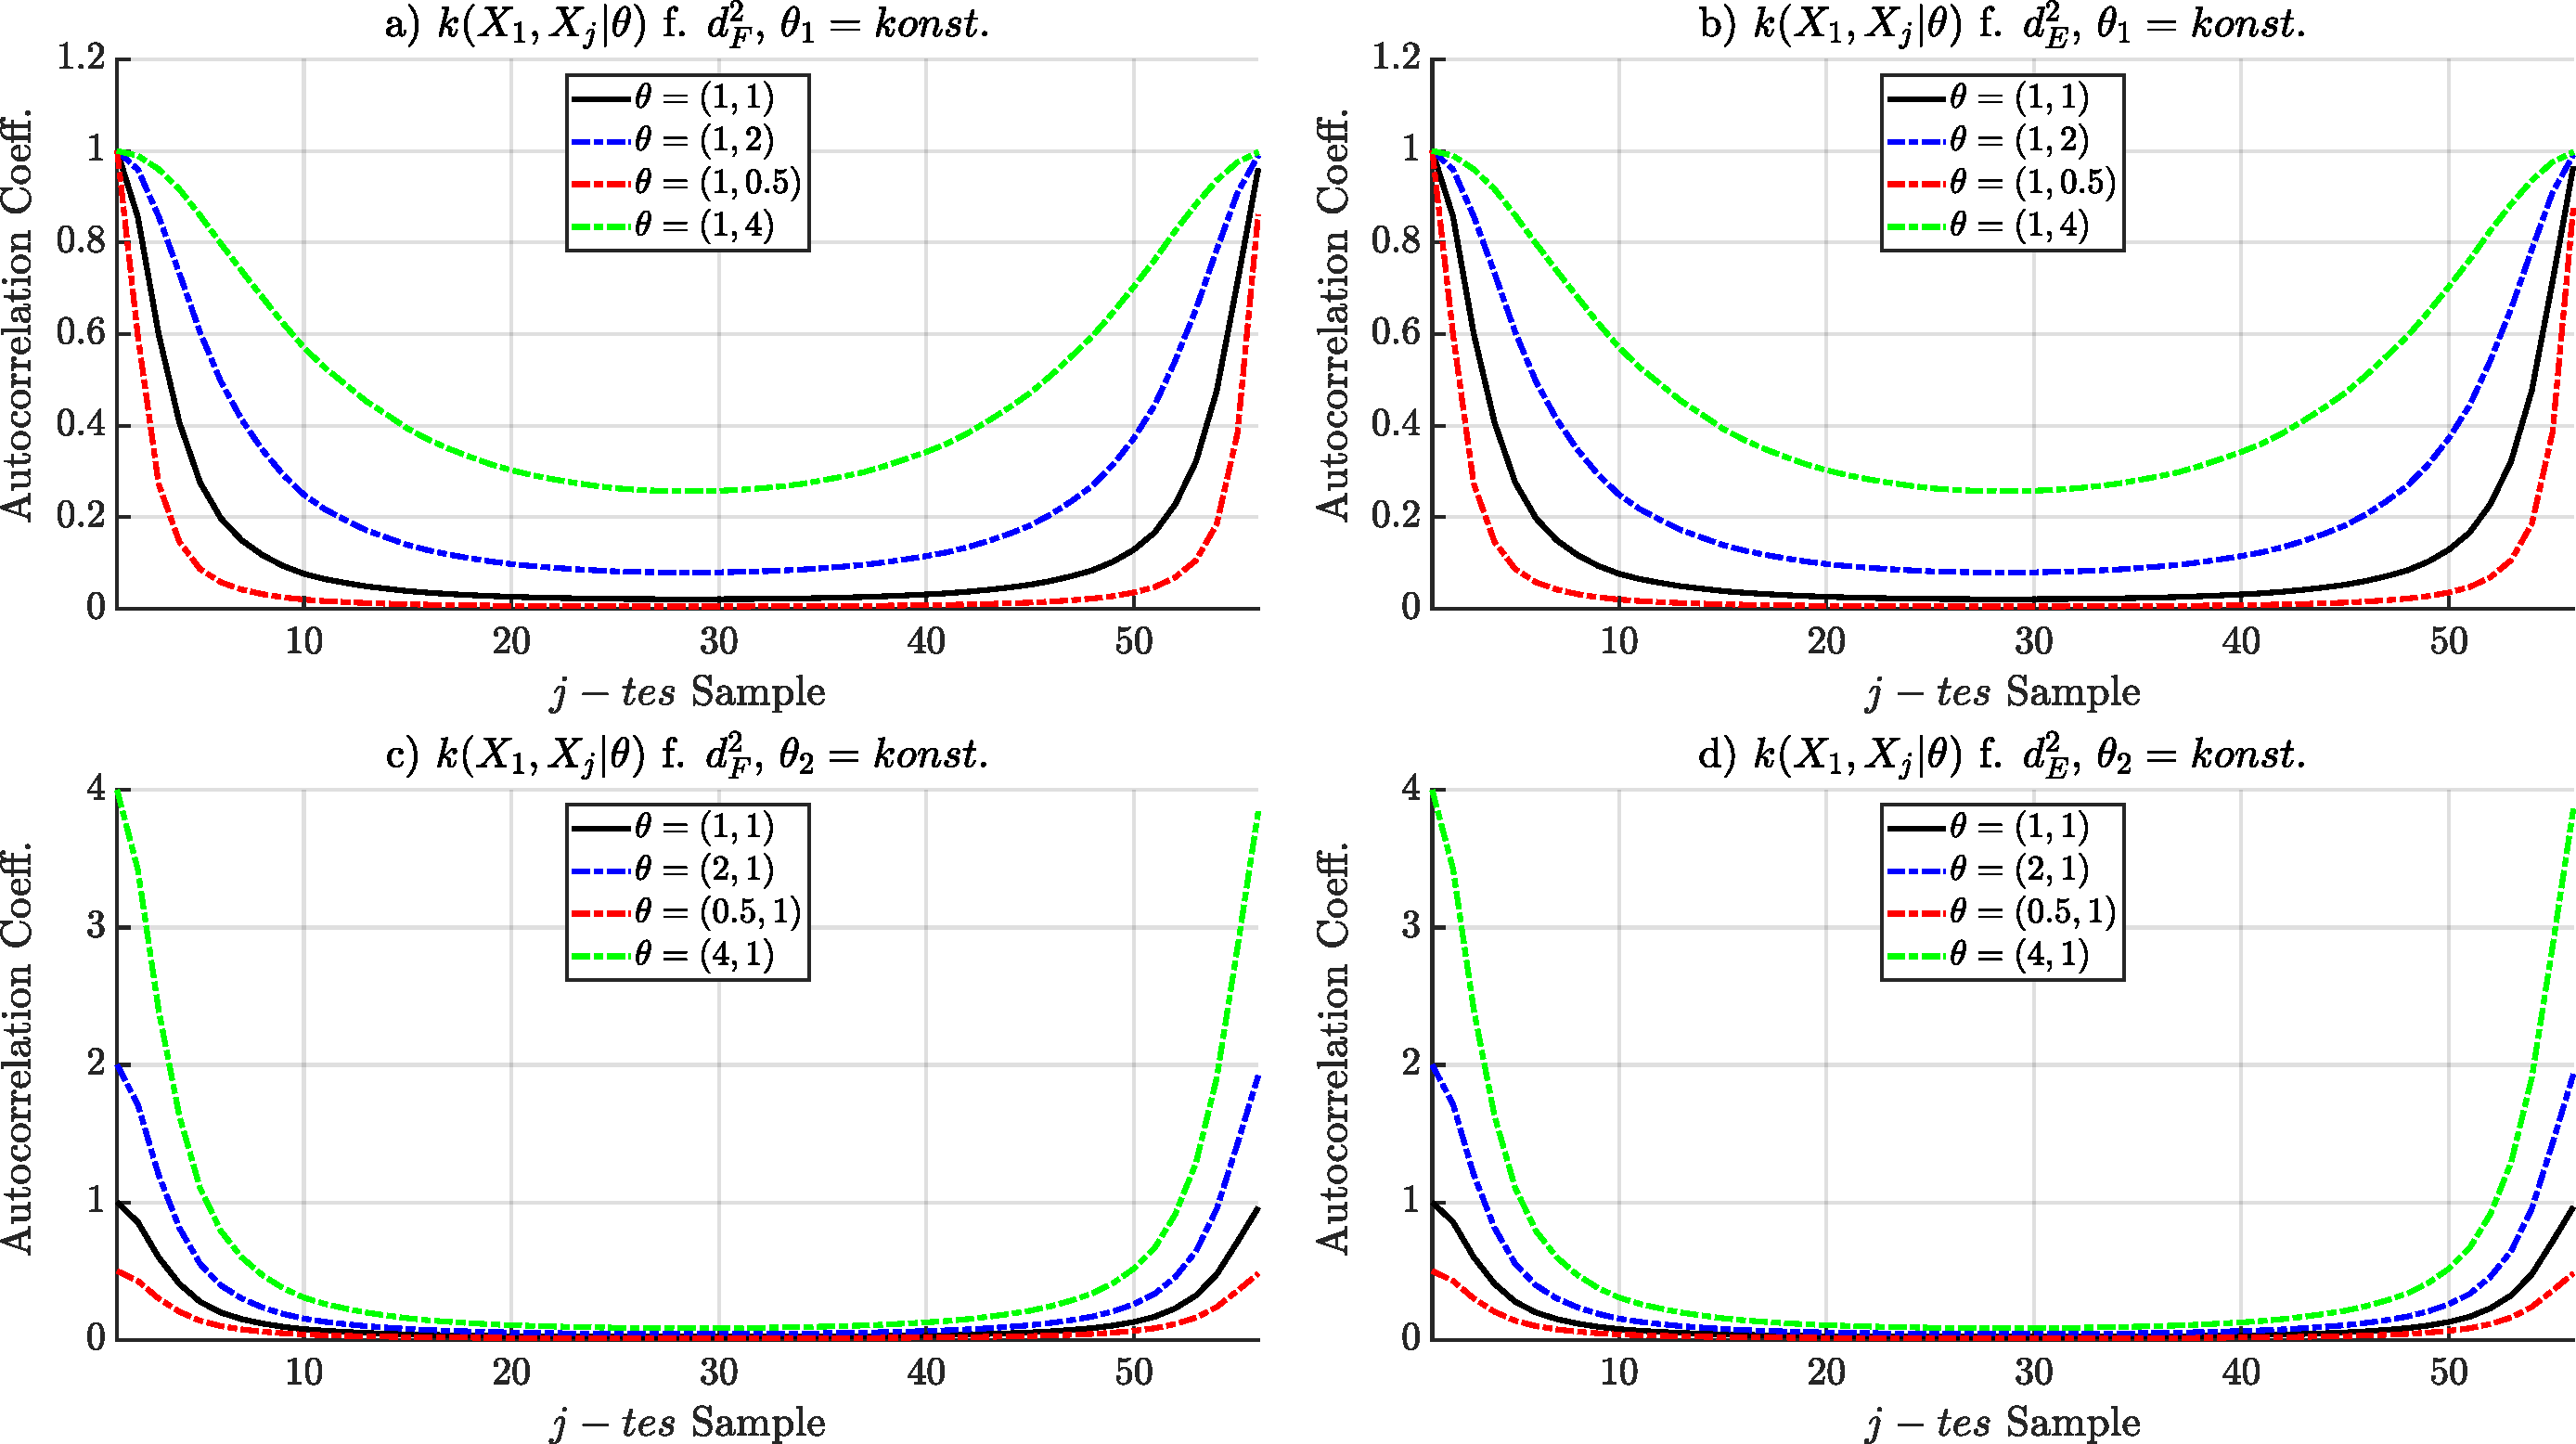
\includegraphics[width=\linewidth]{chapters/images/4-EuOExp/Vergleich-Kovarianzfunktionen}
\caption[Kovarianzfunktionen im Vergleich]{Kovarianzfunktionen im Vergleich für variierende Kernel-Parameter $\theta = (\sigma_f^2, \sigma_l)$ und $N_{Ref} = 56$ Referenzwinkel. Die Kovarianzfunktionen nach \autoref{eq:kfun} mit Frobenius-Norm nach \autoref{eq:df2} als Abstandsfunktion in den Abbildungen a) bzw. c) und mit euklidischer Norm nach \autoref{eq:de2innorm} in den Abbildungen b) bzw. d). Die Abbildungen a) und b) zeigen beide Funktionen mit variabler Längenskalierung $\theta_2 = \sigma_l$ und ausgeschalteter Höhenskalierung mit $\theta_1 = \sigma_f^2 = 1$. Vice versa sind beide Funktionen in den Abbildungen c) und d) gezeigt. Trainingsdaten basieren in a) und c) auf Matrizen. In b) und d) basieren Trainingsdaten auf Vektoren bzw. Skalare. Grafik nachempfunden aus \cite{Lang2014}.}
\label{fig:vergleich-kovarianzfunktionen}
\end{figure}


\clearpage
\begin{figure}[tph]
\centering
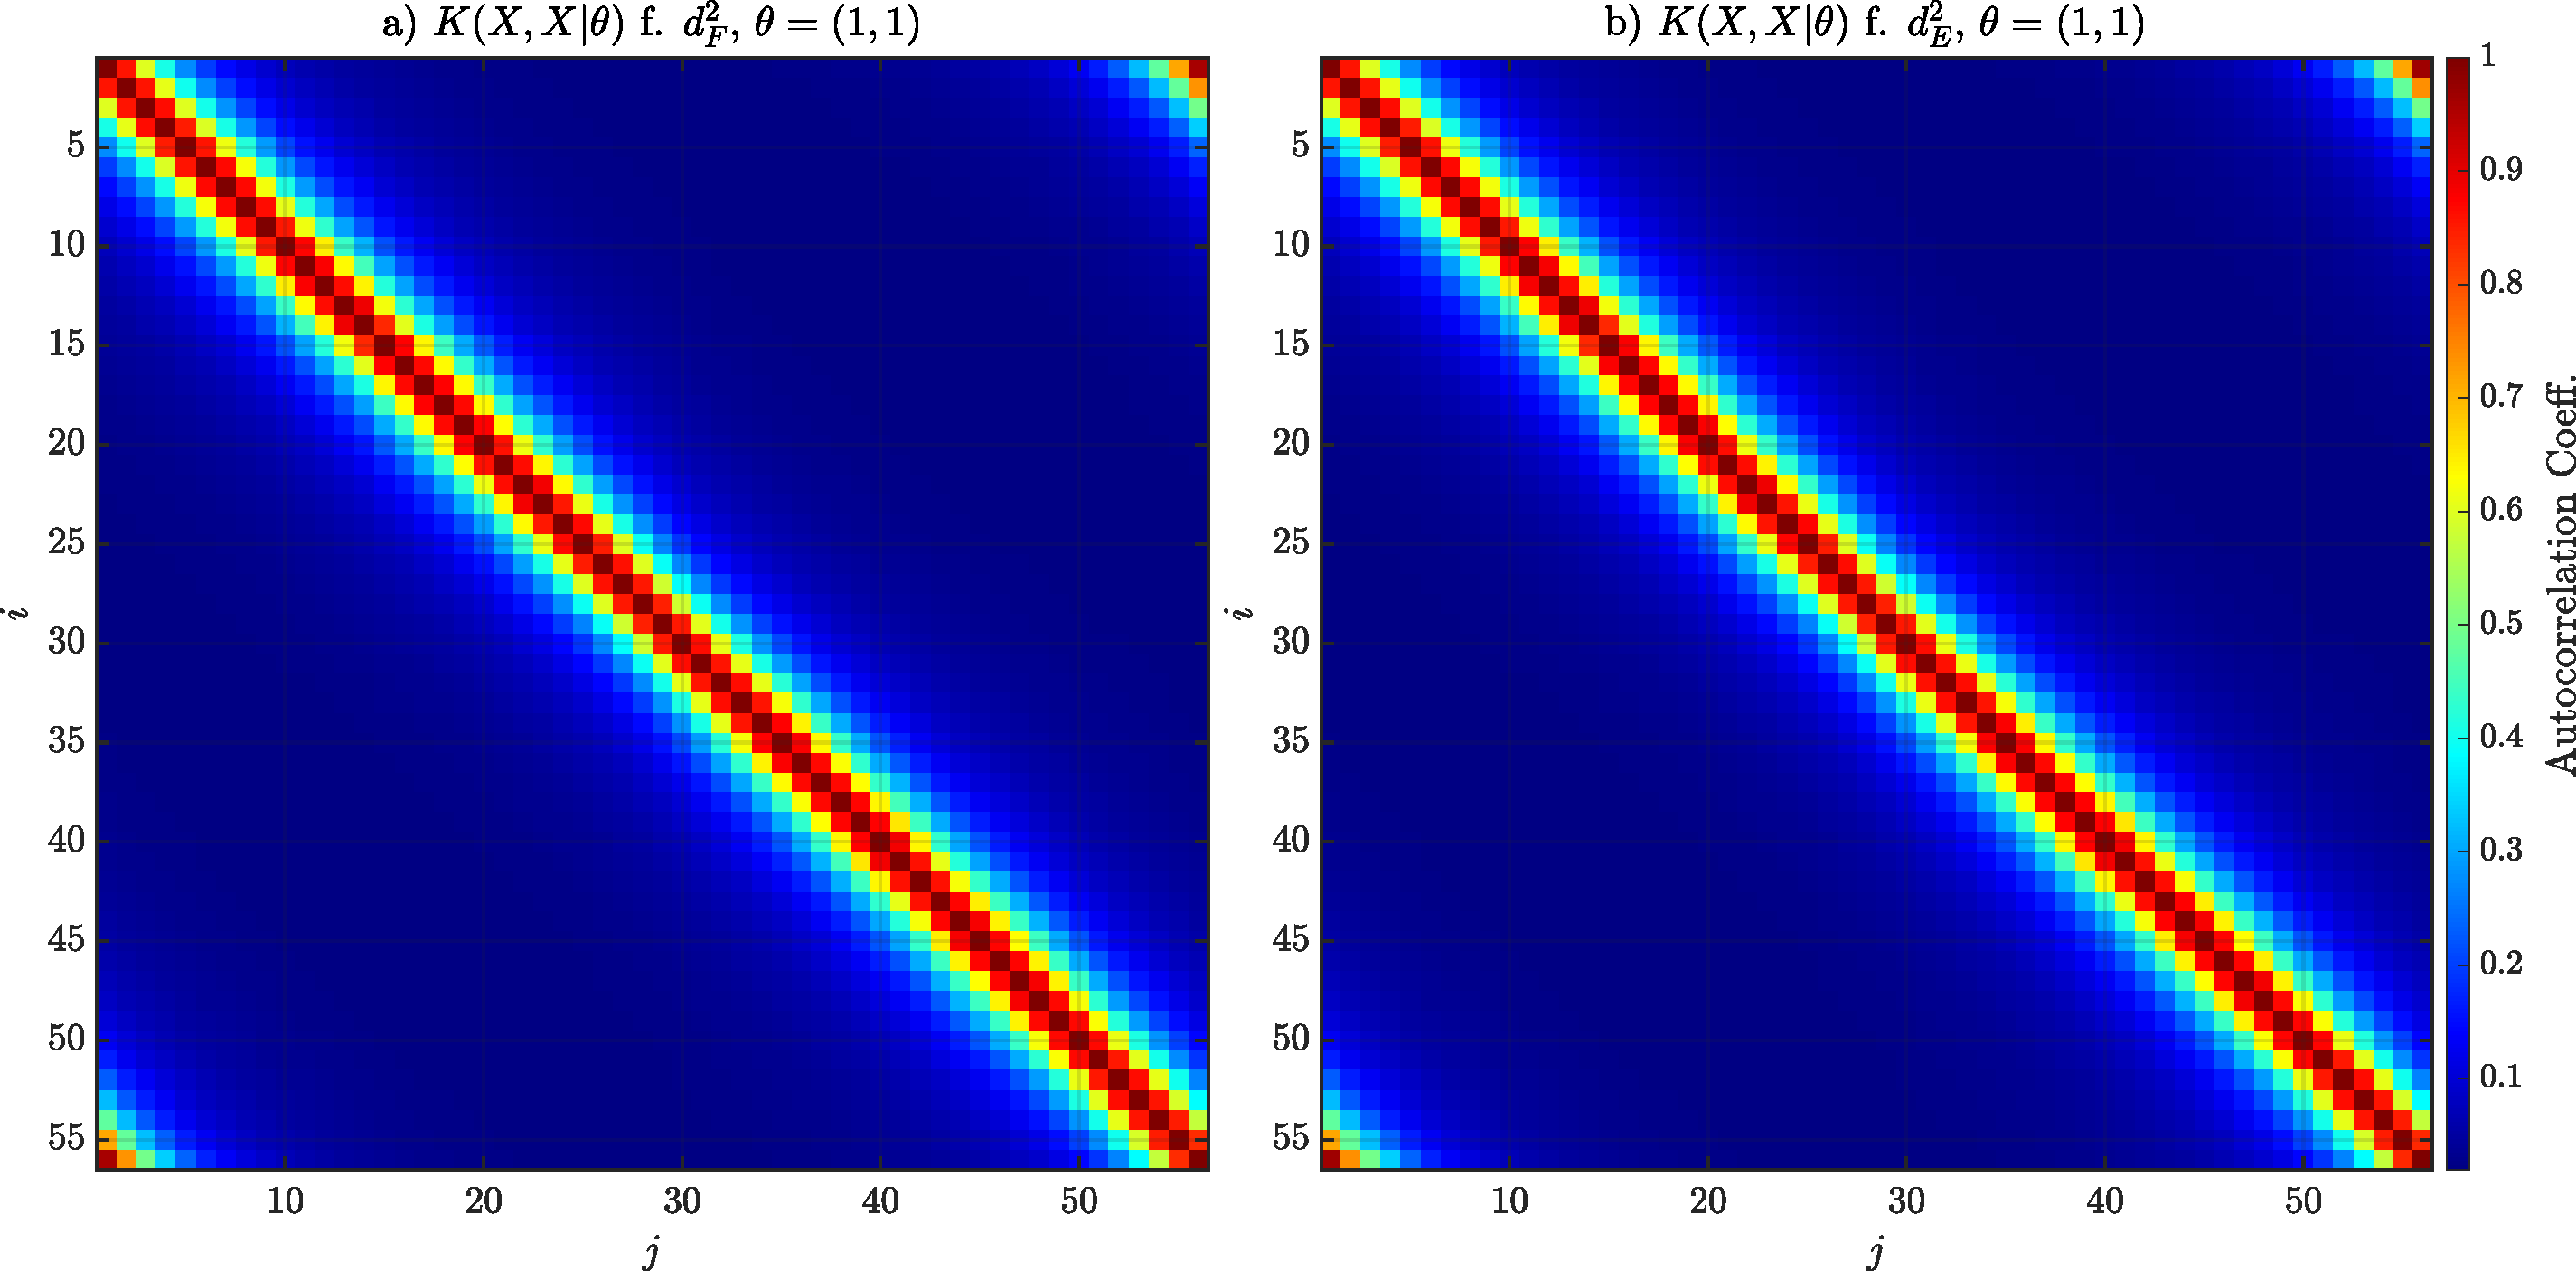
\includegraphics[width=\linewidth]{chapters/images/4-EuOExp/Vergleich-Kovarianzmatrizen}
\caption[Gegenüberstellung der Kovarianzmatrizen]{Gegenüberstellung der Kovarianzmatrizen bei ausgeschalteter Längen- und Höhenskalierung mit $\theta = (1,1)$ und $N_{Ref} = 56$ Referenzwinkel. In Abbildung a) nach Kovarianzfunktion mit Frobenius-Norm als Abstandsfunktion und in Abbildung b) mit euklidischen Abstand, siehe \autoref{eq:kfun}. In a) basieren Trainingsdaten auf Matrizen in b) auf Vektoren bzw. Skalare.}
\label{fig:vergleich-kovarianzmatrizen}
\end{figure}


\clearpage
\begin{figure}[tph]
\centering
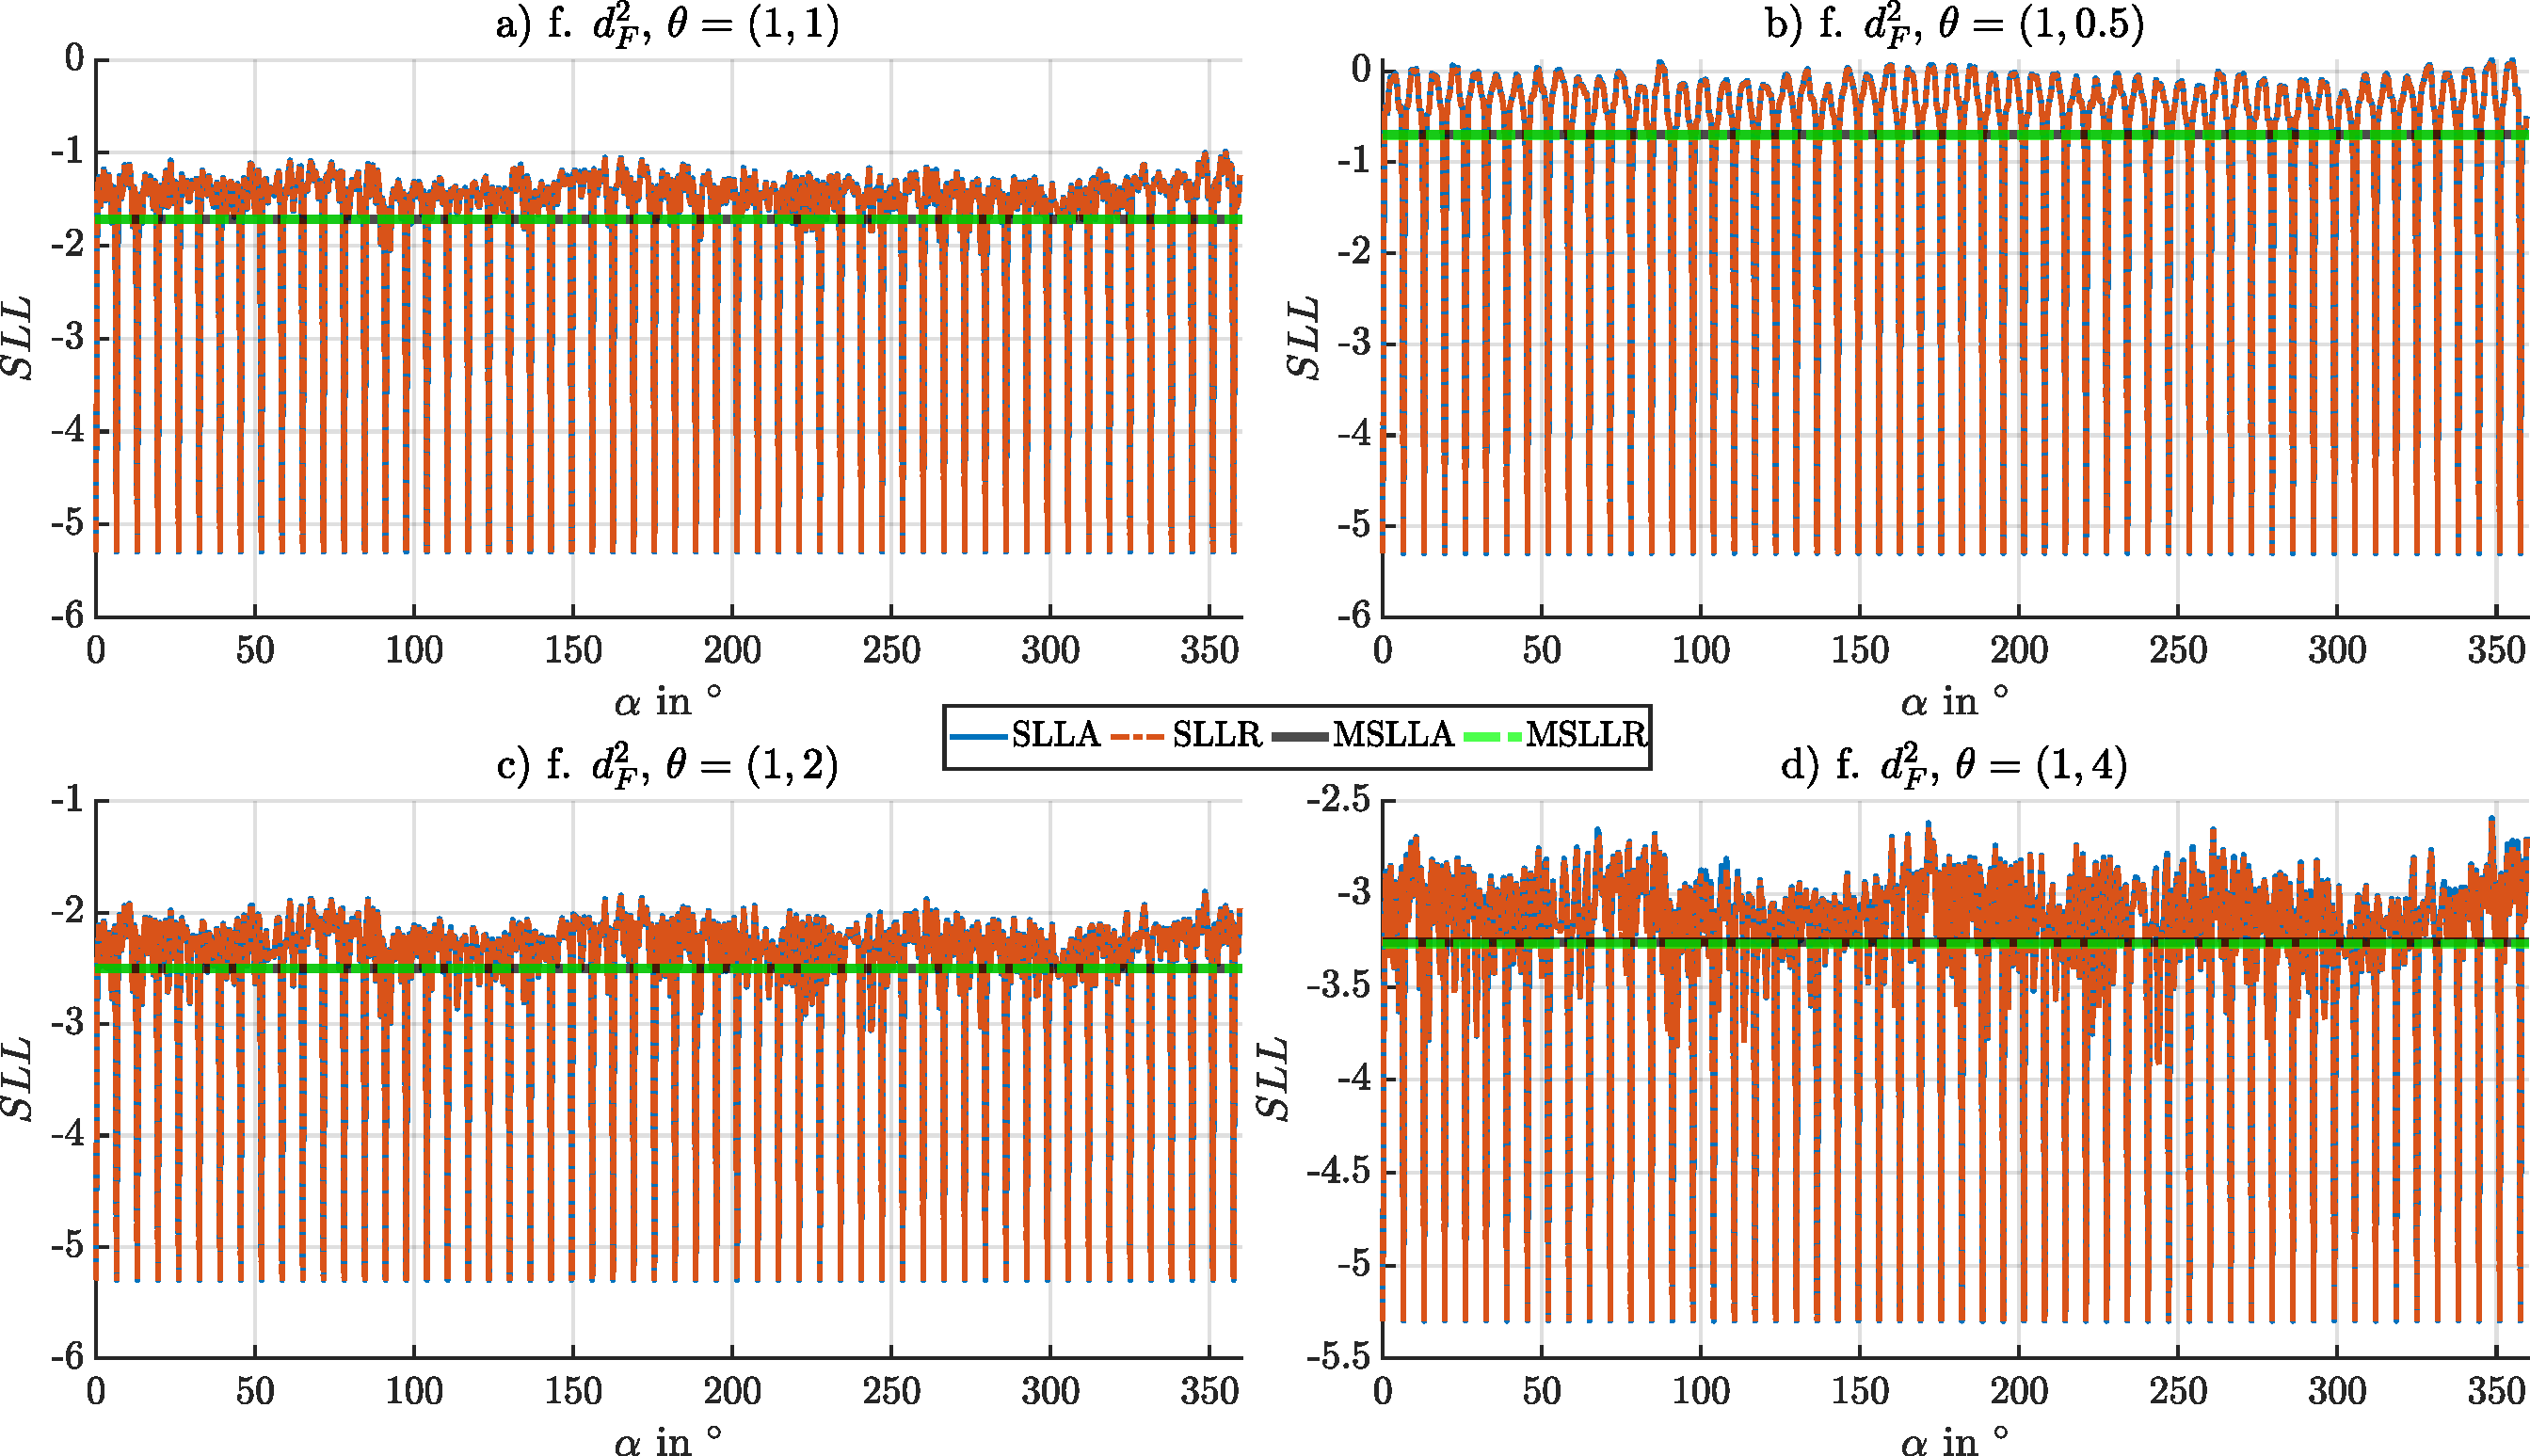
\includegraphics[width=\linewidth]{chapters/images/4-EuOExp/Vergleich-QFC-SLL}
\caption[Modellgeneralisierung mit Frobenius-Norm als Abstandfunktion]{Modellgeneralisierung mit Frobenius-Norm als Abstandfunktion nach \autoref{eq:kfun} und Trainingsdaten basierend auf Matrizen für $N_{Ref} = 56$ Referenzwinkel. Die Berechnungen zur Modellgeneralisierung erfolgten mit einem Testdatensatz für eine volle Rotation des Gebermagneten mit $720$ gleichverteilten Simulationswinkeln bei einer Winkelauflösung von $\SI{0,5}{\degree}$. Die Position des Sensors und die Magnetverkippung sind in beiden Datensätzen identisch. Variiert wurde die Längenskalierung $\theta_2 = \sigma_l$ bei ausgeschalteter Höhenskalierung $\theta_1 = \sigma_f^2 = 1$ der Kovarianzfunktion. Die Modellgeneralisierung wird über den standardisierten logarithmischen Verlust (engl. Loss) $SLL$ a. u. des Modells bewertet \cite{Rasmussen2006}. In Bezug auf Winkel (engl. Angle) mit $SLLA$ und Radius $SLLR$. Als Schwellwertkriterium dient die Mittlung (engl. Mean) der beiden Verluste zu $MSLLA$ und $MSLLR$ nach \autoref{eq:bayesopt}. Das Rauschniveau ist konstant mit $\sigma_n^2 = 10^{-6}$.}
\label{fig:vergleich-qfc-sll}
\end{figure}


\clearpage
\begin{figure}[tph]
\centering
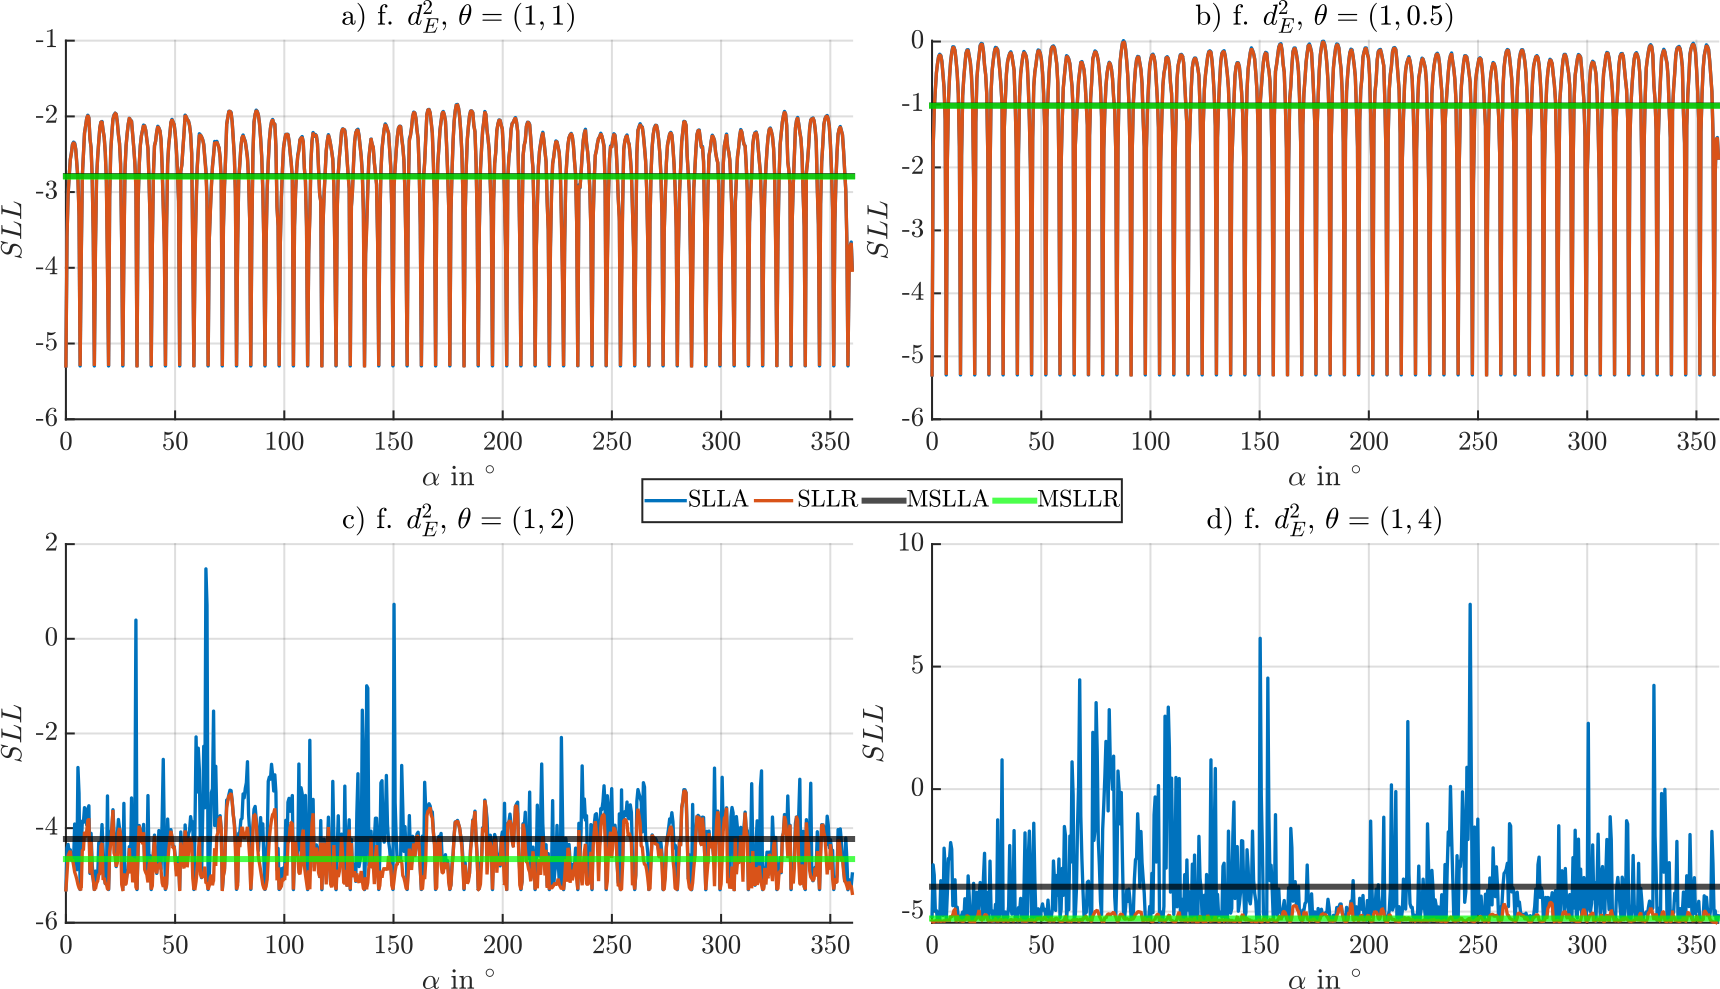
\includegraphics[width=\linewidth]{chapters/images/4-EuOExp/Vergleich-QFCAPX-SLL}
\caption[Modellgeneralisierung mit euklidischer Abstandsfunktion]{Modellgeneralisierung mit euklidischer Abstandsfunktion nach \autoref{eq:kfun} und Trainingsdaten basierend auf Vektoren bzw. Skalare für $N_{Ref} = 56$ Referenzwinkel. Die Berechnungen zur Modellgeneralisierung erfolgten mit einem Testdatensatz für eine volle Rotation des Gebermagneten mit $720$ gleichverteilten Simulationswinkeln bei einer Winkelauflösung von $\SI{0,5}{\degree}$. Die Position des Sensors und die Magnetverkippung sind in beiden Datensätzen identisch. Variiert wurde die Längenskalierung $\theta_2 = \sigma_l$ bei ausgeschalteter Höhenskalierung $\theta_1 = \sigma_f^2 = 1$ der Kovarianzfunktion. Die Modellgeneralisierung wird über den standardisierten logarithmischen Verlust (engl. Loss) $SLL$ a. u. des Modells bewertet \cite{Rasmussen2006}. In Bezug auf Winkel (engl. Angle) mit $SLLA$ und Radius $SLLR$. Als Schwellwertkriterium dient die Mittlung (engl. Mean) der beiden Verluste zu $MSLLA$ und $MSLLR$ nach \autoref{eq:bayesopt}. Das Rauschniveau ist konstant mit $\sigma_n^2 = 10^{-6}$.}
\label{fig:vergleich-qfcapx-sll}
\end{figure}
\clearpage


% !TEX root = ../thesis.tex
% adjust number of reference angles
% @author Tobias Wulf
%

\section{Anpassung der Referenzwinkelanzahl}\label{sec:exp2}


\textbf{Zweck:} Das Experiment soll einen Bereich abstecken für die Wahl der Anzahl für gleichverteilte Referenzwinkel. Dafür wird die äußere Modelloptimierung über das Rauschniveau nach \autoref{alg:bayesopt} ausgeschaltet und ein konstantes Rauschniveau $\sigma_n^2$ vorgeben. Das Regressionsmodell wird daher nur für die Längen- und Höhenskalierung $\theta = (\sigma_f^2, \sigma_l)$ der Kovarianzfunktion optimiert, siehe \autoref{alg:fminconopt}. Verglichen wird das Regressionsmodell für euklidischen Abstand nach \autoref{eq:de2innorm} und \autoref{eq:kfun} einmal ohne unterstützende Mittelwertbildung über Polynome (Zero-Mean) und mit Polynombildung ersten Grades, siehe \autoref{eq:hfun} bis \autoref{eq:gprmean}. Diese wirkt als eine Offset- und Amplitudenkorrektur der Messwerten. Es werden absolute mittlere und maximale Winkelfehler in Abhängigkeit der Referenzwinkelanzahl verglichen. Zusätzliche wird die Berechnungsdauer einer Winkelvorhersage in Abhängigkeit der Referenzwinkelanzahl bzw. Trainingspunkte aufgenommen. Im besten Fall stellt sich heraus, dass das Mittelwert freie Verfahren gleich oder besser ist gegenüber dem Polynom gestützten Verfahren. Die Umsetzung des letzteren Verfahrens ist deutlich aufwendiger zu gestalten und birgt einige numerischer Fehleranfälligkeiten und Hürden, die es in den Griff zu bekommen gilt.

\textbf{Durchführung:} Es werden zwei Modelle mit euklidischer Abstandfunktion initialisiert und Trainiert, jeweils mit und ohne unterstützendes Mittelwertpolynom. Jedes der beiden Modelle wird mit pro Durchgang mit gleichem Trainingsdaten trainiert und anschließend die Skalierung der Kovarianzfunktion in Länge und Höhe entsprechend der Trainingsdaten getrimmt. Danach wird die Zeit gemessen, die es benötigt einen Simulationswinkel zu vorherzusagen. Jeweils getrennt für beide Modelle. Zum Ende des Durchgangs werden absolute Winkelfehler auf eine volle Rotation mit einem Testdatensatz über $720$ Winkeln bei einer Auflösung von $\SI{0,5}{\degree}$ berechnet und für mittlere sowie maximale Winkelfehler über die gesamte Rotation ausgewertet. Ebenfalls für beide Modelle. Der Durchgang wird für jeden zur Verfügung stehenden Trainingsdatensatz wiederholt. Der Testdatensatz bleibt für jeden Durchgang gleich. Alle Datensätze sind für die gleiche Position des Sensors und bei gleicher Verkippung des Magneten zuvor prozessiert worden.

\textbf{Erzeugte Datensätze:} Es sind für das Experiment 12 Trainingsdatensätze mit unterschiedlicher Referenzwinkelanzahl und ein Testdatensatz erzeugt worden. Alle Datensätze korrespondieren in Position und Verkippung.

\textbf{Matlab-Skript:} compareCpuTimeVsError.m, siehe \autoref{mcode:comparecputimevserror}.


\clearpage


\textbf{Abweichende Parameter von \autoref{tab:sim-params-exp}:}

\begin{itemize}
	\item TrainingsOptions: nAngles: $\left\{ 8, 16, 24, 32, 40, 48, 60, 80, 120, 240, 360, 720 \right\}$
	\item GRPOptions: kernel : 'QFCAPX'
	\item GPROptions: mean: 
	\begin{itemize}
		\item[a.] 'zero'
		\item[b.] 'poly'
	\end{itemize}
\end{itemize}

\textbf{Ergebnisse:} Die Ergebnisse des Experiments sind grafisch in \autoref{fig:timings-vs-errors} ausgewertet. Berechnungszeiten für einen Simulationswinkel a) sowie mittlerer b) und maximaler c) absoluter Winkelfehler bei voller Rotation sind in Abhängigkeit der Referenzwinkelanzahl in den Trainingsdatensätzen aufgetragen.

\textbf{Beobachtungen:} Die Messung der Berechnungszeit für eine Simulationswinkelvorhersage in a) ergibt, dass beide Implementierungskonfigurationen annähernd gleich schnell sind und die Rechenzeit bis eine Referenzwinkelanzahl von $N_{Ref} = 80$ mit leichten Abweichungen konstant bleibt. Für eine Referenzwinkelanzahl von $N_{Ref} > 80$ nimmt die Rechenzeit für beide Varianten gleichermaßen exponentiell zu. Für absolute mittlere und maximale Winkelfehler unterscheiden sich die mittelwertfreie und Polynom gestützte Variante nur bei $N_{ref} = 8$. Dort liefert jeweils die mittelwertfreie Variante den geringeren Winkelfehler. Für eine Referenzwinkelanzahl $N_{Ref} > 8$ liefern beide Variationen einen annähernd gleichen Winkelfehler. Bei einer Referenzwinkelanzahl von $N_{Ref} = 48$ gibt es eine Sprungstelle für den mittleren und maximalen Winkelfehler, beide mittlerer sowie maximaler Winkelfehler verringern sich ungefähr um die Hälfte. Der Winkelfehler bleibt nach dem Sprung konstant und schwankt nur noch minimal. Dieser Bereich (2) ist in den Abbildungen b) und c) grau unterlegt und weißt im Vergleich zu Bereich (1) weniger Fehlerdynamik für nachfolgende Optimierungsschritte auf. Der interessante Bereich (1) für eine weitere Optimierung über das Rauschniveau $\sigma_n^2$ nach \autoref{alg:bayesopt} ist in a), b) und c) grün unterlegt. Diesen gilt es im weiteren Verlauf anzupassen und die Sprungstelle in b) und c) zu verkleinern oder auszulöschen.


\clearpage
\begin{landscape}
\begin{figure}[tbph]
	\centering
	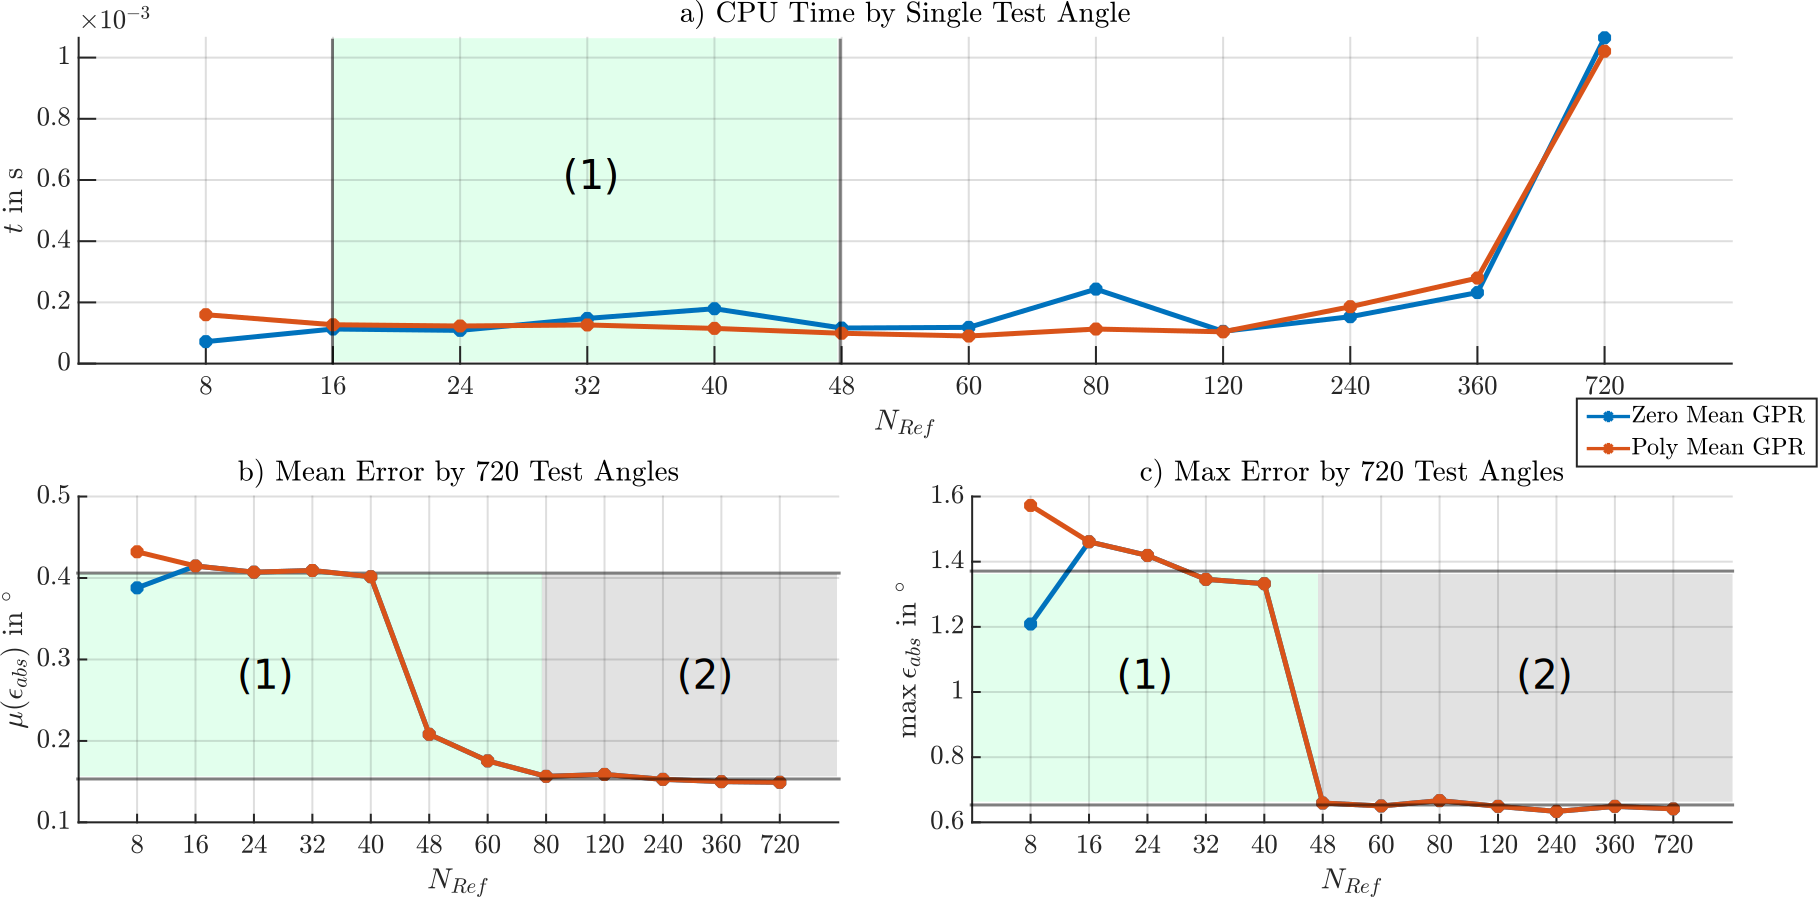
\includegraphics[width=\linewidth]{chapters/images/4-EuOExp/Timings-vs-Errors}
	\caption[Variation der Referenzwinkelanzahl bei konstantem Rauschniveau]{Variation der Referenzwinkelanzahl bei konstantem Rauschniveau $\sigma_n^2 = 10^{-6}$. Es wird die Implementierung des Regressionsmodell nach \autoref{eq:kfun} mit euklidischen Abstand nach \autoref{eq:de2innorm}, jeweils ohne (Zero Mean GPR) und mit Mittelwertunterstützung (Poly Mean GPR) in Abhängigkeit der Referenzwinkelanzahl $N_{Ref}$ verglichen. Dafür wird in a) die Berechnungszeit eines Simulationswinkel gemessen und in b) der absolute mittlere Winkelfehler, sowie in c) der absolute maximale Winkelfehler auf eine volle Rotation ausgewertet. Die jeweiligen initiierten Modellvariation sind für ihre Kovarianzfunktionsparameter $\theta = (\sigma_f^2,\sigma_l)$ getrimmt nach \autoref{alg:fminconopt}. Die Optimierung des Rauschniveaus $\sigma_n^2$ nach \autoref{alg:bayesopt} ist ausgeschaltet. Modelltrainingsdaten basieren hier für beide Varianten auf Vektoren bzw. Skalare.}
	\label{fig:timings-vs-errors}
\end{figure}
\end{landscape}


\clearpage

	
% !TEX root = ../thesis.tex
% adjust noise level
% @author Tobias Wulf
%

\section{Anpassung des Rauschniveaus für Noisy-Observation}\label{sec:exp3}


\textbf{Zweck:} Das Experiment ist eine Fortsetzung zum \autoref{sec:exp2} und schaltet zusätzlich zur Trimmung der Kovarianzfunktion nach \autoref{alg:fminconopt} die äußere Modelloptimierung über das Rauschniveau $\sigma_n^2$ nach \autoref{alg:bayesopt} ein. Es dient primär zur weiteren Anpassung der Referenzwinkelanzahl und untersucht sekundär die Möglichkeit zur Winkelfehlerminimierung unter Berücksichtigung der gemachten Beobachtungen im \autoref{sec:exp2}. Ziel ist es hier, einen Kompromiss zu finden, bestehend aus brauchbarer Generalisierung und akzeptablen Winkelfehler bei möglichst geringer Referenzwinkelanzahl. Dafür werden für jeden Durchgang Modellverlust, absoluter mittlerer Winkelfehler sowie der maximale Winkelfehler auf eine volle Rotation mit $720$ Simulationswinkeln bei einer Auflösung von $\SI{0,5}{\degree}$ berechnet. Dafür wird wie in \autoref{sec:exp2} das Regressionsmodell für euklidischen Abstand nach \autoref{eq:de2innorm} und \autoref{eq:kfun} in beiden Varianten einmal als mittelwertfreies Modell und Mittelwert-unterstütztes Modell betrieben. Es wird der in \autoref{fig:timings-vs-errors} grün gekennzeichnete Bereich (1) näher untersucht.

\textbf{Durchführung:} Die Durchführung ist aus \autoref{sec:exp2} zu entnehmen. Änderungen in der Durchführung beziehen sich auf die Ausführungen zur Ermittlung der Berechnungszeit für eine Winkelvorhersage, diese ist durch die Berechnung der Modellverluste für Winkel ersetzt.

\textbf{Erzeugte Datensätze:} Es sind für das Experiment 24 Trainingsdatensätze mit unterschiedlicher Referenzwinkelanzahl und ein Testdatensatz erzeugt worden. Alle Datensätze korrespondieren in Position und Verkippung.

\textbf{Matlab-Skript:} compareNoiseOptAbility.m, siehe \autoref{mcode:comparenoiseoptability}.

\textbf{Abweichende Parameter von \autoref{tab:sim-params-exp}:}

\vspace{5mm}
\begin{table}[htp]
	\centering
	\resizebox{\textwidth}{!}{
		\begin{tabular}{l l c l}
			\toprule
			\textbf{Parametergruppe} & \textbf{Parameter} & \textbf{Wert}         & \textbf{Kurzbeschreibung}                  \\ \midrule
			TrainingOptions          & nAngles            & $\left[8:1:31\right]$ & Simulationswinkelanzahl inkrementiert um 1 \\ \hline
			GPROptions               & kernel             & 'QFCAPX'              & Indikator für zweite Kernel-Variante       \\
			                         & mean               & 'zero'/ 'poly'        & Indikator Mittelwertpolynom variiert       \\ \bottomrule
		\end{tabular}}
	\caption{Abweichende Simulationsparameter im Experiment zur Rauschniveauanpassung.}
	\label{tab:params-exp3}
\end{table}


\clearpage


\textbf{Ergebnisse:} Die Ergebnisse des Experiments sind grafisch in \autoref{fig:msll-vs-errors} ausgewertet. Modellverlust für Winkel in a), sowie mittlerer b) und maximaler c) absoluter Winkelfehler. Alle drei durchgeführten Berechnungen erfolgten für jeden Durchgang mit voller Rotation um $720$ Testwinkel und sind in Abhängigkeit der Referenzwinkelanzahl in den Trainingsdatensätzen aufgetragen.

\textbf{Beobachtungen:} Die Betrachtung der Generalisierung in \autoref{fig:msll-vs-errors} a) über den mittleren standardisierten logarithmischen Verlust $MSLL$ (hier für Winkelverluste) zeigen, dass bei zunehmender Referenzwinkelanzahl $N_{Ref}$ sich die Generalisierung verbessert und das Regressionsmodell besser auf von den Trainingsdaten abweichende Datensätze reagiert. Auftretende Schwankungen in der Generalisierung a) bilden sich gleichermaßen in den Winkelfehlern b) und c) ab. In Bezug auf die gemachten Beobachtungen aus \autoref{sec:exp2} und \autoref{fig:timings-vs-errors} Bereich (1) ist es gelungen, den mittleren und maximalen Winkel weiter zu drücken. Der mittlere Winkelfehler in b) und maximale Winkelfehler in c) schwingen sich der Generalisierung folgend auf die Winkelfehlerniveaus aus \autoref{fig:timings-vs-errors} b) und c) ein. Ein möglicher Kompromiss aus Generalisierung, Winkelfehler und möglichst geringer Referenzwinkelanzahl ist für $N_{Ref} = 17$ in \autoref{fig:msll-vs-errors} markiert.


\clearpage
\begin{figure}[tph]
	\centering
	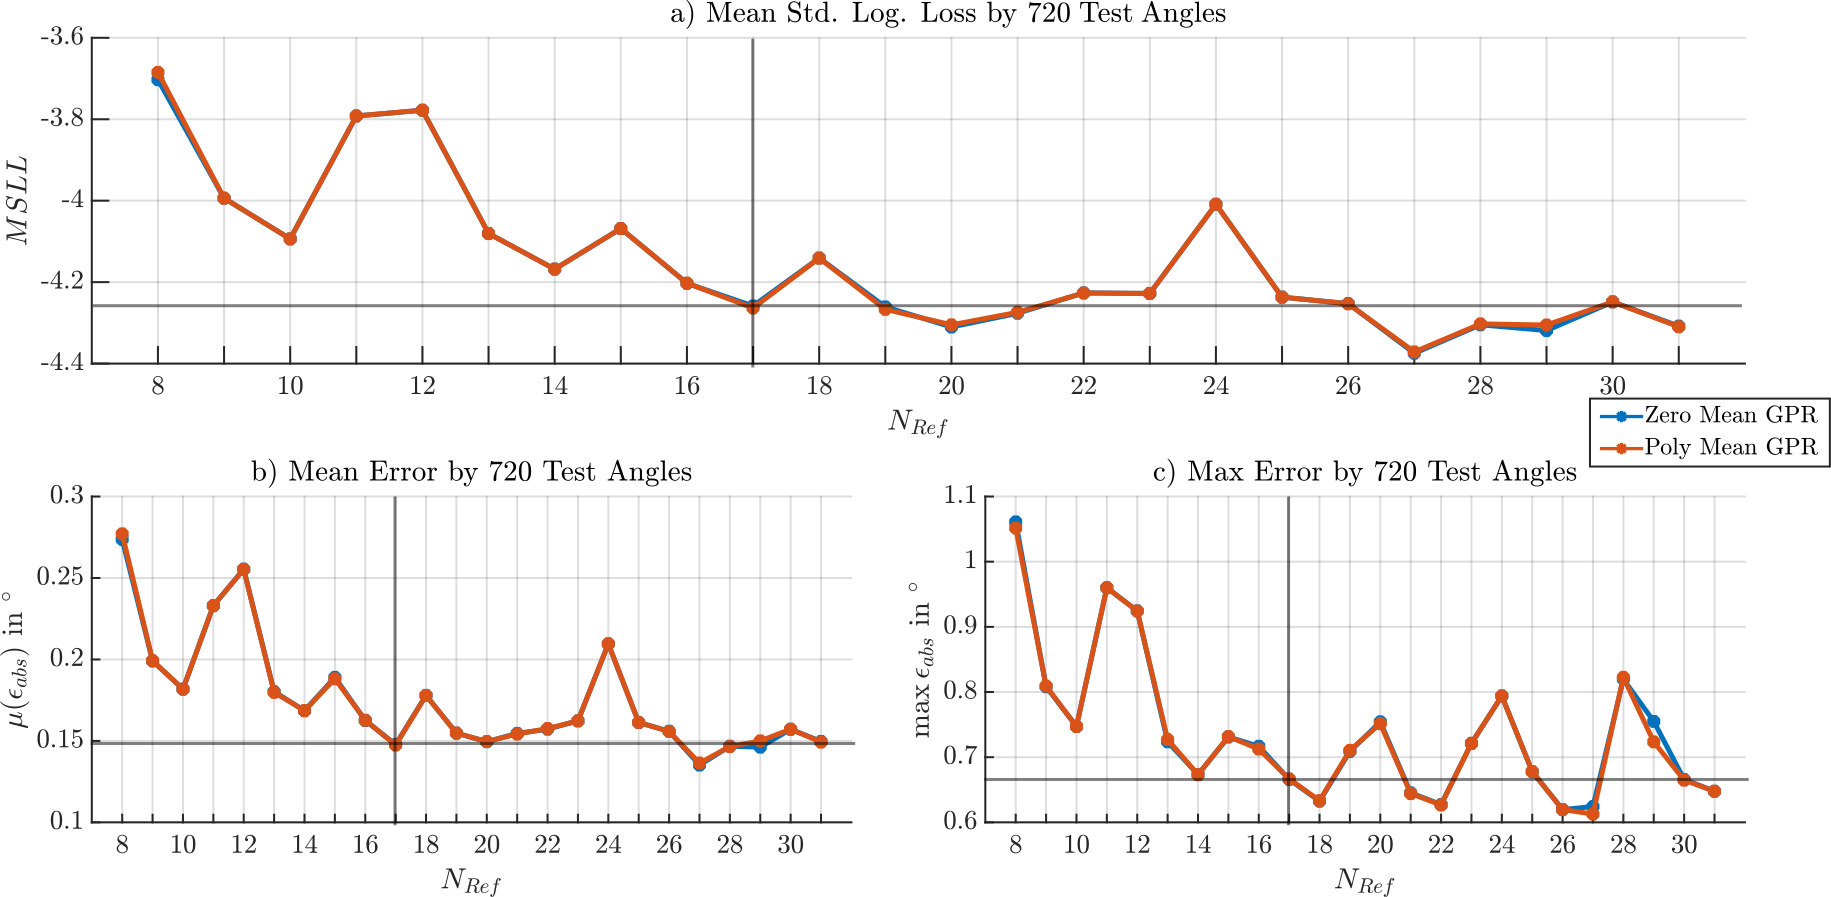
\includegraphics[width=\linewidth]{chapters/images/4-EuOExp/MSLL-vs-Errors}
	\caption[Variation der Referenzwinkelanzahl mit Optimierung des Rauschniveau]{Variation der Referenzwinkelanzahl mit Optimierung des Rauschniveaus $\sigma_n^2$ nach \autoref{alg:bayesopt}. Es wird die Implementierung des Regressionsmodell nach \autoref{eq:kfun} mit euklidischen Abstand nach \autoref{eq:de2innorm}, jeweils ohne (Zero Mean GPR) und mit Mittelwertunterstützung (Poly Mean GPR) in Abhängigkeit der Referenzwinkelanzahl $N_{Ref}$ verglichen. Dafür wird in a) die Modellgeneralisierung über den mittleren standardisierten logarithmischen Verlust (engl. Loss) $MSLL$ a. u. nach \autoref{eq:bayesopt} bewertet. Die Verlustberechnung ist für Winkelverluste konfiguriert. In b) folgen der absolute mittlere Winkelfehler sowie in c) der absolute maximale Winkelfehler. Alle drei Berechnungen sind jeweils für jeden Schritt auf eine volle Rotation durchgeführt worden. Modelltrainingsdaten basieren hier auf Vektoren bzw. Skalare.}
	\label{fig:msll-vs-errors}
\end{figure}


\clearpage


% !TEX root = ../thesis.tex
% adjust parameter limits
% @author Tobias Wulf
%

\section{Anpassung der Parametergrenzen}\label{sec:exp4}

\textbf{Zweck:} Das Experiment besitzt einen veranschaulichenden Charakter und soll zeigen, wie der Rechenaufwand für die Optimierungen nach \autoref{alg:fminconopt} und \autoref{alg:bayesopt} verringert werden kann. Dafür werden die Parameter der Kovarianzfunktion in Abhängigkeit der Modellplausibilitäten nach \autoref{eq:fmincon} untersucht und das Rauschniveau in Verbindung mit den mittleren Modellverlust $MSLL$ nach \autoref{eq:bayesopt} gezeigt. Ziel ist es, die Durchlaufzahl für die äußere Optimierung über das Rauschniveau und \autoref{alg:bayesopt} zu verkürzen und dabei die Generalisierung des Modells aufrechtzuerhalten.
Aussagen zur Modellgeneralisierung und Modellanpassung auf den Trainingsdaten sind den Anhängen \autoref{sec:gpropt} und \autoref{sec:gprgen} zu entnehmen.

\textbf{Durchführung:} Das Experiment wir in zwei Durchgängen durchgeführt. In beiden wird Regressionsmodell nach \autoref{eq:de2innorm} und \autoref{eq:kfun} mittels \autoref{alg:fminconopt} und \autoref{alg:fminconopt} optimiert und anschließend ein Parameter-Sweep für die Parameter der Kovarianzfunktion in Abhängigkeit der Modellplausibilität nach \autoref{eq:fmincon} durchgeführt. Der Parameter-Sweep wird für jeden Parameter für eine zusätzliche Dekade neben den Parametergrenzen ausgeführt. Der erste Durchgang wird mit der Default-Konfiguration aus \autoref{tab:sim-params-exp} ausgeführt. Danach werden die Parametergrenzen angepasst, die Durchlaufzahl verringert und das Experiment wiederholt.

\textbf{Erzeugte Datensätze:} Jeweils ein Trainings- und Testdatensatz mit korrespondierender Position des Sensors und Verkippungswinkel des Magneten.

\textbf{Matlab-Skript:} investigateKernelParameters.m, siehe \autoref{mcode:investigatekernelparameters}

\textbf{Abweichende Parameter von \autoref{tab:sim-params-exp}:}


\vspace{5mm}
\begin{table}[htp]
	\centering
	\resizebox{\textwidth}{!}{
		\begin{tabular}{l l c l}
			\toprule
			\textbf{Parametergruppe} & \textbf{Parameter}  & \textbf{Wert}        & \textbf{Kurzbeschreibung}                          \\ \midrule
			TrainingOptions          & nAngles             & $17$                 & Simulationswinkelanzahl angepasst                  \\ \hline
			GPROptions               & kernel              & 'QFCAPX'             & Indikator für zweite Kernel-Variante               \\
			                         & $\sigma_f^2$-Bounds & $(1, 10)$            & Parameter-Bounds $\theta_1 = \sigma_f^2$ angepasst \\
			                         & $\sigma_l$-Bounds   & $(10, 30)$           & Parameter-Bounds $\theta_2 = \sigma_l$ angepasst   \\
			                         & $\sigma_n^2$-Bounds & $(10^{-6}, 10^{-4})$ & Parameter-Bounds $\sigma_n^2$ angepasst            \\
			                         & OptimRuns           & $10$                 & Durchlaufanzahl äußere Optimierung verringert      \\
			                         & mean                & 'zero'               & Mittelwertpolynom ausgeschaltet                    \\ \bottomrule
		\end{tabular}}
	\caption{Abweichende Simulationsparameter im Experiment zur Parametergrenzenanpassung.}
	\label{tab:params-exp4}
\end{table}


\clearpage


\textbf{Ergebnisse:} Die Ergebnisse des Durchgangs sind grafisch in \autoref{fig:qfcapx-z-n17-bounds} und \autoref{fig:qfcapx-z-n17-opt} ausgewertet. \autoref{fig:qfcapx-z-n17-bounds} zeigt die Anpassung der Parametergrenzen für die Optimierungsalgorithmen und \autoref{fig:qfcapx-z-n17-opt} veranschaulicht die Verringerung der Durchlaufzahl für die äußere Optimierung.



\textbf{Beobachtungen:} Die engeren Parametergrenzen für die Parameter der Kovarianzfunktion stecken ein engeres Suchfeld für das innere Minimierungsproblem ab, zu sehen in \autoref{fig:qfcapx-z-n17-bounds} b). Der Algorithmus findet das Minimum und besitzt noch genügend Freiraum, sodass die Parametergrenzen nicht verletzt werden. In Teil a) der \autoref{fig:qfcapx-z-n17-bounds} schafft es die äußere Optimierung den Schwellwert für die Generalisierung entsprechend gut abzusenken. Es gibt ebenfalls keine Verletzungen der Parametergrenzen. Das Minimum ist extrem und Fehlergrenzen des Algorithmus können nach wenigen Schritten im Bereich des Minimums stark eingegrenzt werden. Die \autoref{fig:qfcapx-z-n17-opt} beobachtet die Minimum-Kriterien der Algorithmen in Bezug auf die Anzahl der Durchläufe. Abbildung a) für die äußere Optimierung und b) sowie c) für die innere Optimierung. Die innere Optimierung wird bei jedem Durchlauf der äußeren wiederholt, siehe \autoref{sub:gpr-pro}. Zu sehen ist der letzte Durchlauf der inneren Optimierung in b) und c). Die äußere Optimierung schafft es nach acht Durchläufen einen stabilen Wert für die Generalisierung zu erreichen. Im letzten Durchgang der inneren Optimierung sind die optimalen Parameter nach fünf Durchgängen gefunden. Die Innere Optimierung benötigt eine gewisse Durchlaufzahl um festzustellen, dass keine markanten Änderungen geschehen und das Minimum gefunden ist. Die äußere Optimierung benötigt die Begrenzung über die Durchlaufzahl.


\clearpage
\begin{figure}[tph]
	\centering
	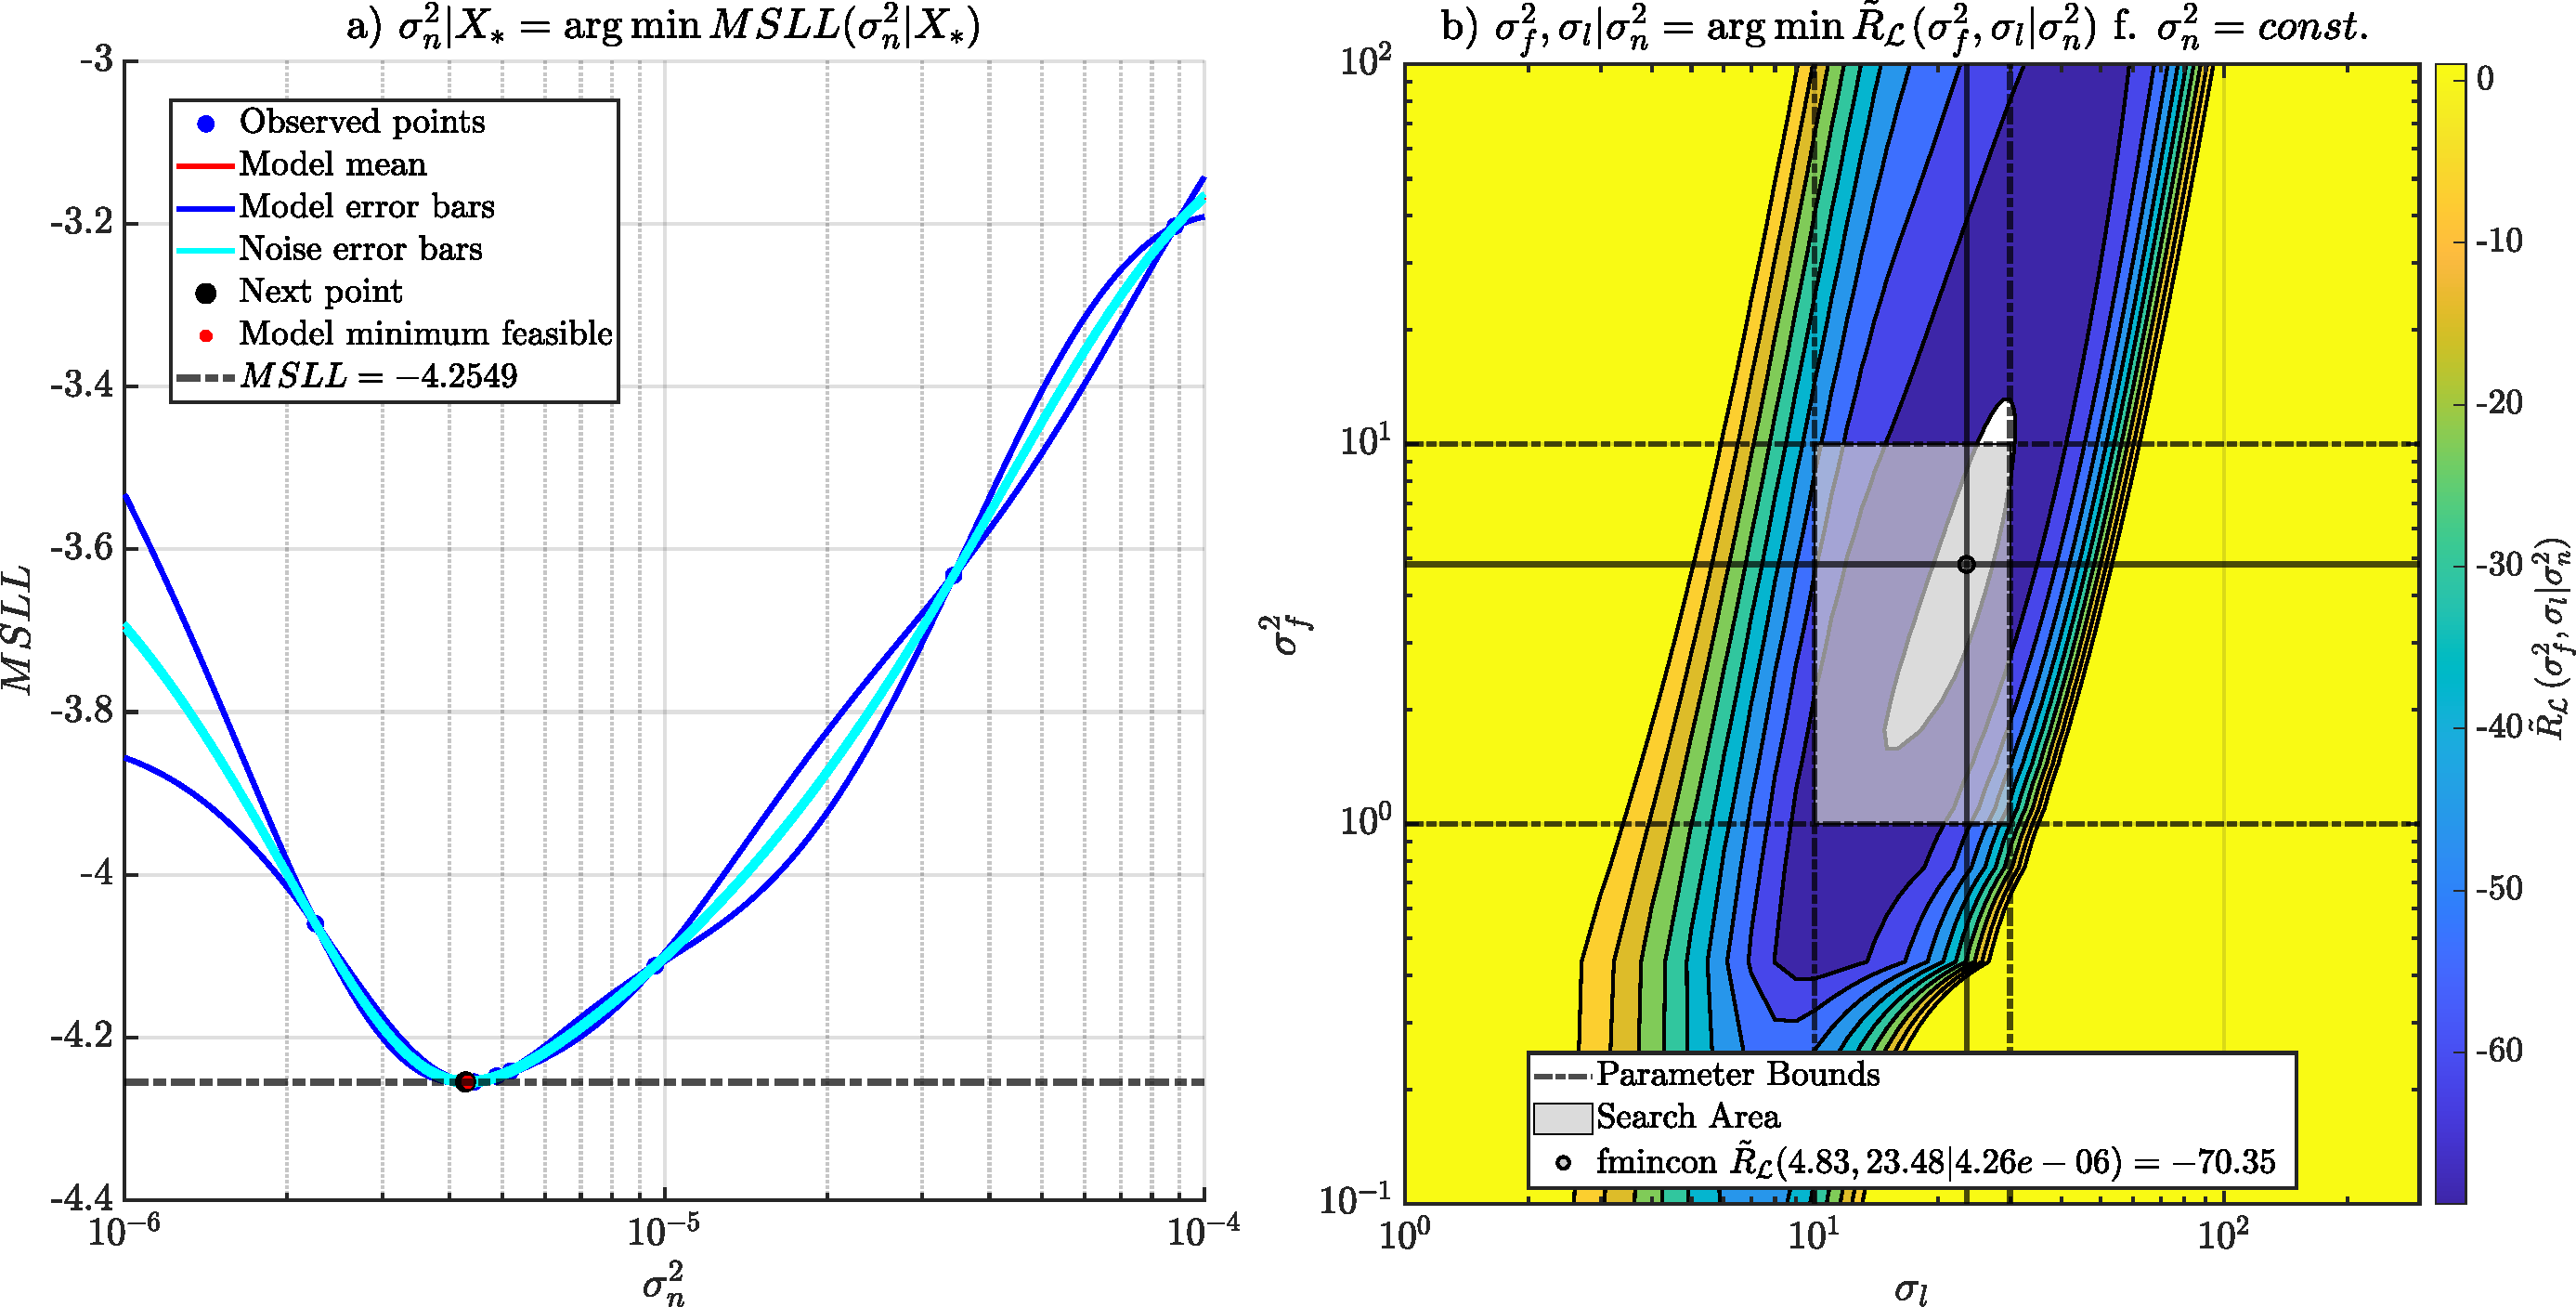
\includegraphics[width=\linewidth]{chapters/images/4-EuOExp/QFCAPX-Z-N17-Bounds}
	\caption[Äußere und innere Modelloptimierung mit angepassten Parametergrenzen]{Äußere und innere Modelloptimierung mit angepassten Parametergrenzen. Die äußere Modelloptimierung in a) für das Rauschniveau $\sigma_n^2$ nach \autoref{alg:bayesopt} und \autoref{eq:bayesopt}. Der mittlere standardisierte logarithmische Verlust $MSLL$ (engl. Loss) ist für alle eingespeisten Testdaten $X_*$ in a) berechnet und ist das Schwellwertkriterium für die Modellgeneralisierung. Die äußere Optimierung gibt das Rauschniveau $\sigma_n^2$ für die innere Optimierung in b) vor. In b) werden basierend auf den eingespeisten Trainingsdaten die Parameter der Kovarianzfunktion nach \autoref{alg:fminconopt} und \autoref{eq:fmincon} getrimmt. Die Optimierung stützt sich auf die Summe der logarithmischen Plausibilitäten (engl. Log. Marginal Likelihoods) für die zu vorhersagenden Cosinus- und Sinus-Funktionen. Beide Optimierungen suchen nach einem Minimum. Hier gezeigt mit angepassten Parametergrenzen in a) für $\sigma_n^2 = (10^{-6}, 10^{-4})$ und in b) für $\sigma_f^2 = (1, 10)$ und $\sigma_l = (10, 30)$. Grafik nachempfunden aus \cite{Rasmussen2006}.}
	\label{fig:qfcapx-z-n17-bounds}
\end{figure}



\clearpage
\begin{figure}[tph]
	\centering
	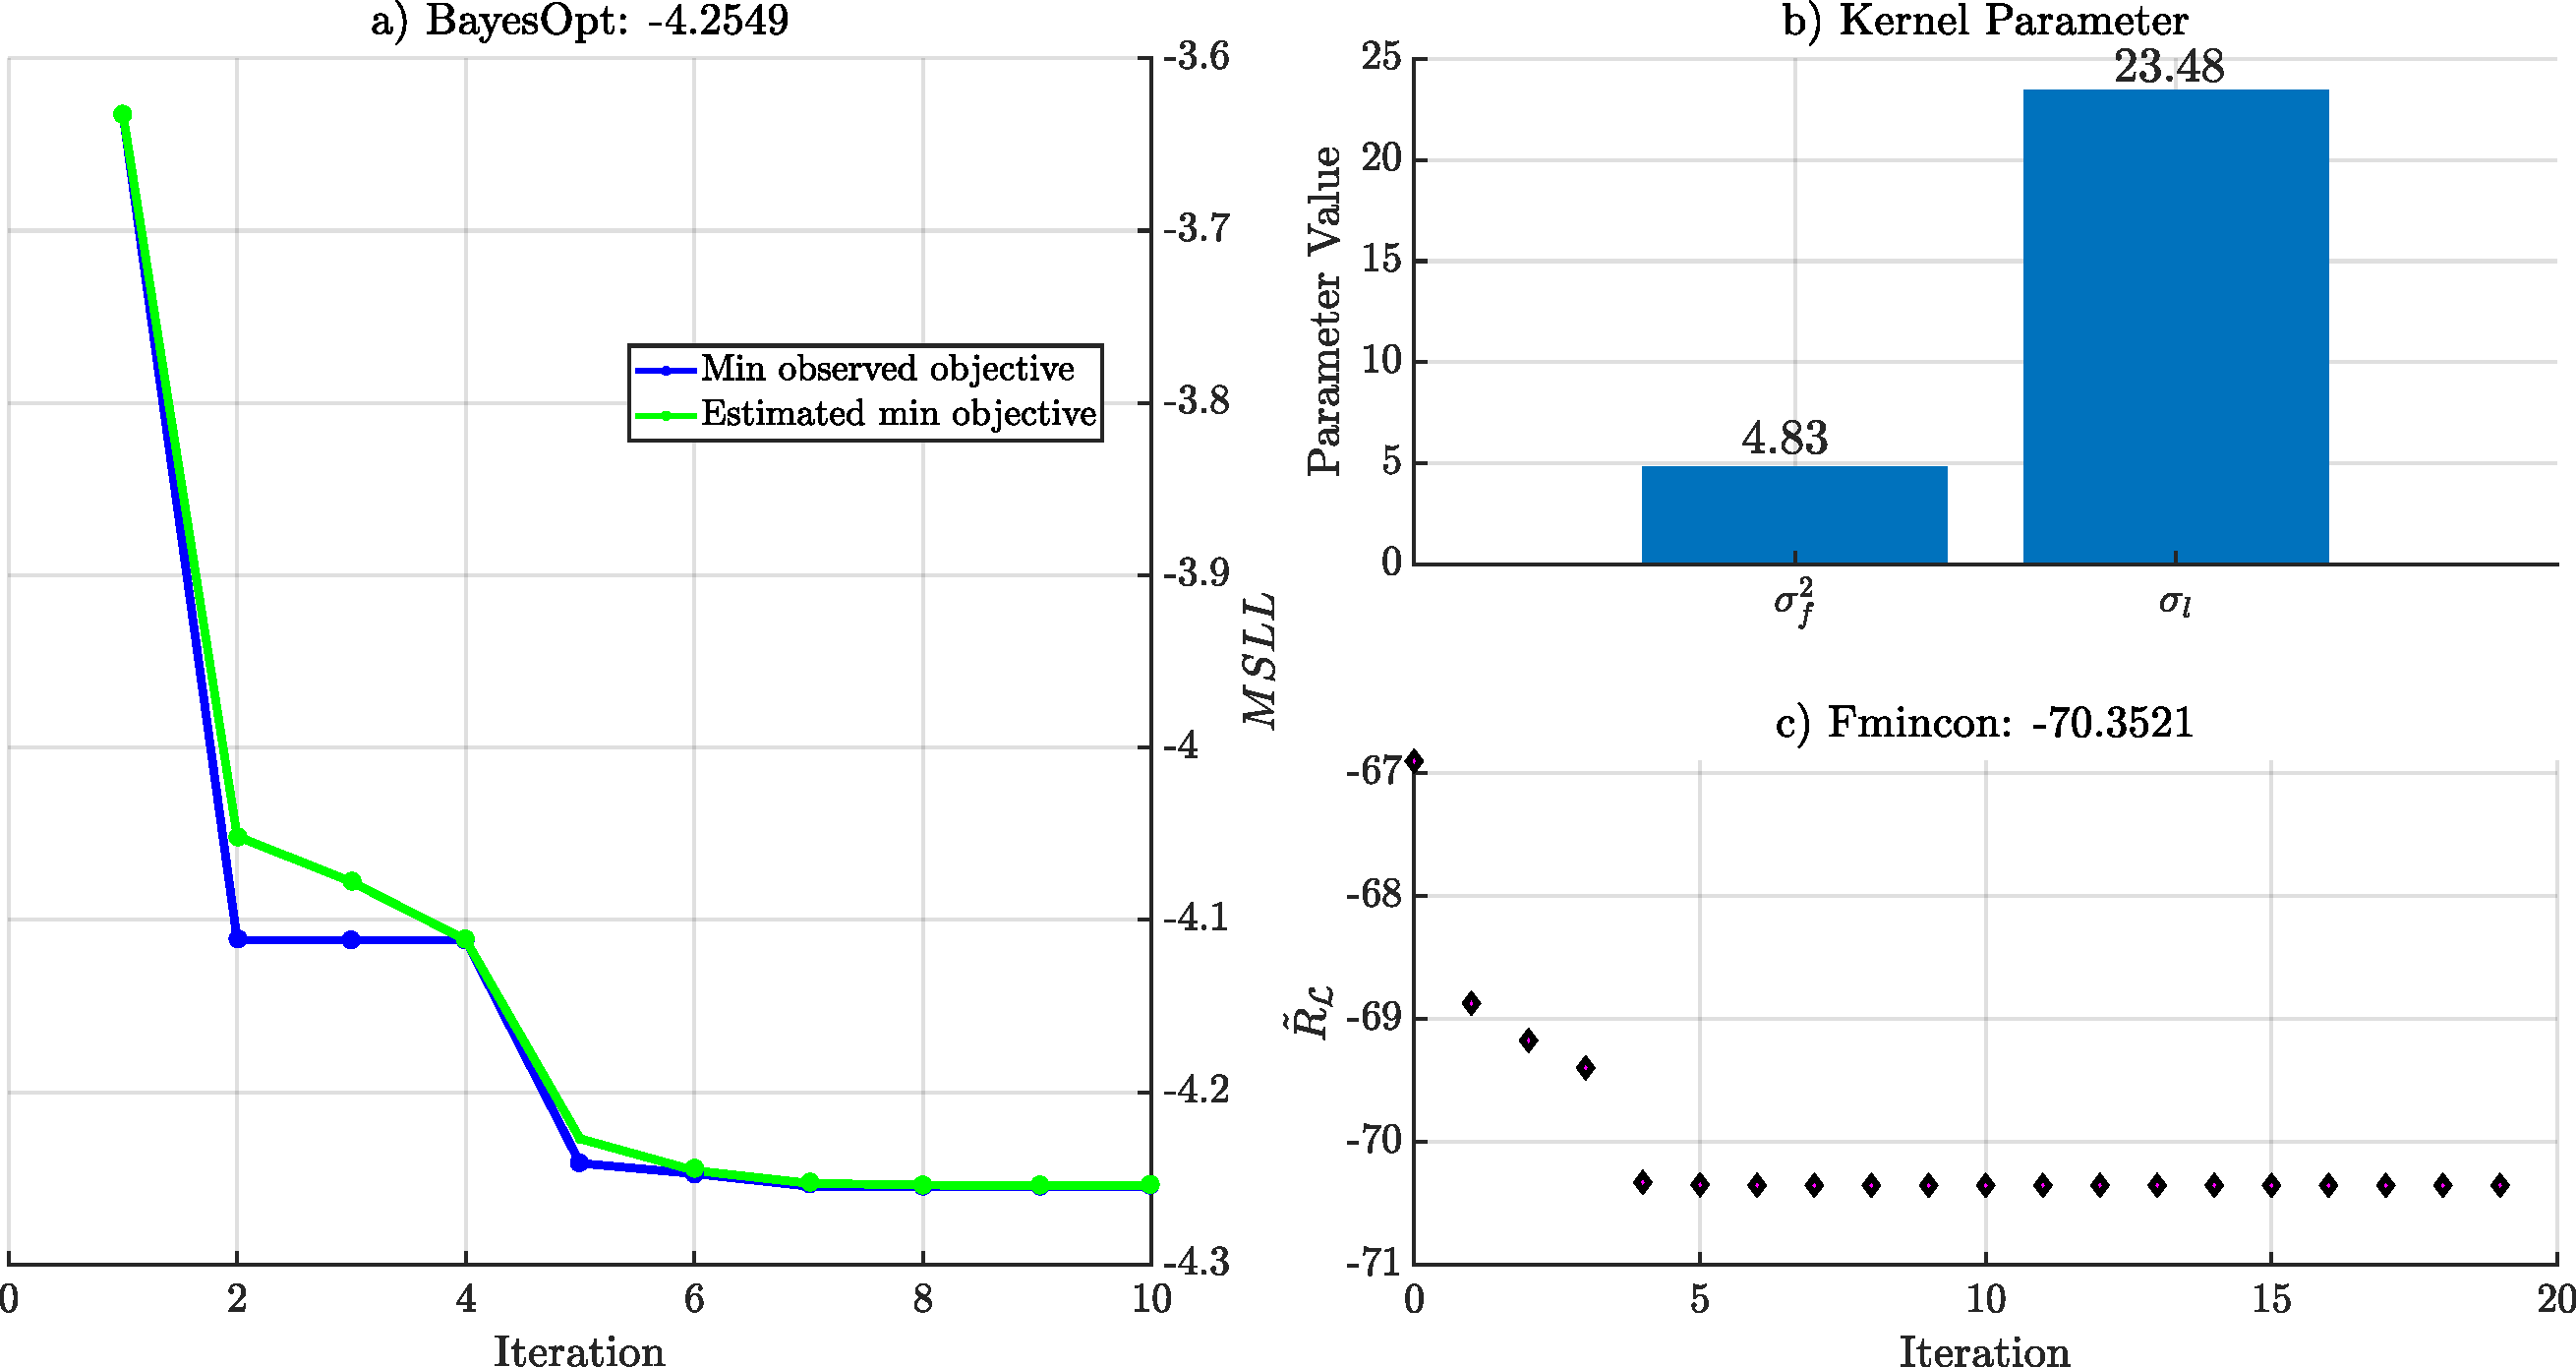
\includegraphics[width=\linewidth]{chapters/images/4-EuOExp/QFCAPX-Z-N17-Opt}
	\caption[Äußere und innere Modelloptimierung mit angepasster Durchlaufzahl]{Äußere und innere Modelloptimierung mit angepasster Durchlaufzahl. Nach Anpassung der Parametergrenzen in \autoref{fig:qfcapx-z-n17-bounds}, ist die Durchlaufzahl für die äußere Modelloptimierung nach \autoref{alg:bayesopt} von $30$ auf $10$ Durchläufe verringert worden. Es gelingt in a) nach $10$ ein stabile Generalisierung mit negativen mittlerem standardisierten logarithmischen Verlust (engl. Loss) $MSLL$ zu finden. Die innere Optimierung in b) und c) nach \autoref{alg:fminconopt} bedarf vorerst keine weiterer Anpassung. Diese ist relativ zur äußeren Optimierung sehr viel schneller, da sie nur mit Trainingsdaten arbeitet.}
	\label{fig:qfcapx-z-n17-opt}
\end{figure}


\clearpage


% !TEX root = ../thesis.tex
% behavior at simple misalignments
% @author Tobias Wulf
%

\section{Verhalten bei einfachen Fehllagen}\label{sec:exp5}

\textbf{Zweck:}

\textbf{Durchführung:}

\textbf{Erzeugte Datensätze:}

\textbf{Matlab-Skript:}

\textbf{Abweichende Parameter von \autoref{tab:sim-params-exp}:}

Referenzposition (0,0,7.5)

\begin{itemize}
	\item TrainingsOptions: nAngles: 17
	\item TrainingsOptions/ TestOptions: xPos/ yPos: $-3:0,25:3$
	\item TrainingsOptions/ TestOptions: zPos: $4,5:0,25:10,5$
	\item TrainingsOptions/ TestOptions: tilt: $0:0,5:12$
	\item GRPOptions: kernel : 'QFCAPX'
	\item $\sigma_f^2$-Bounds: $(0.1,100)$
	\item $\sigma_l$-Bounds: $(1,100)$
	\item $\sigma_n^2$-Bounds: $(10^{-7},10^{-3})$
	\item GPROptions: mean: 'zero'
	\item OptimRuns 30
\end{itemize}


\textbf{Ergebnisse:}

\textbf{Beobachtungen:}

\clearpage
\begin{landscape}
\begin{figure}[tbph]
	\centering
	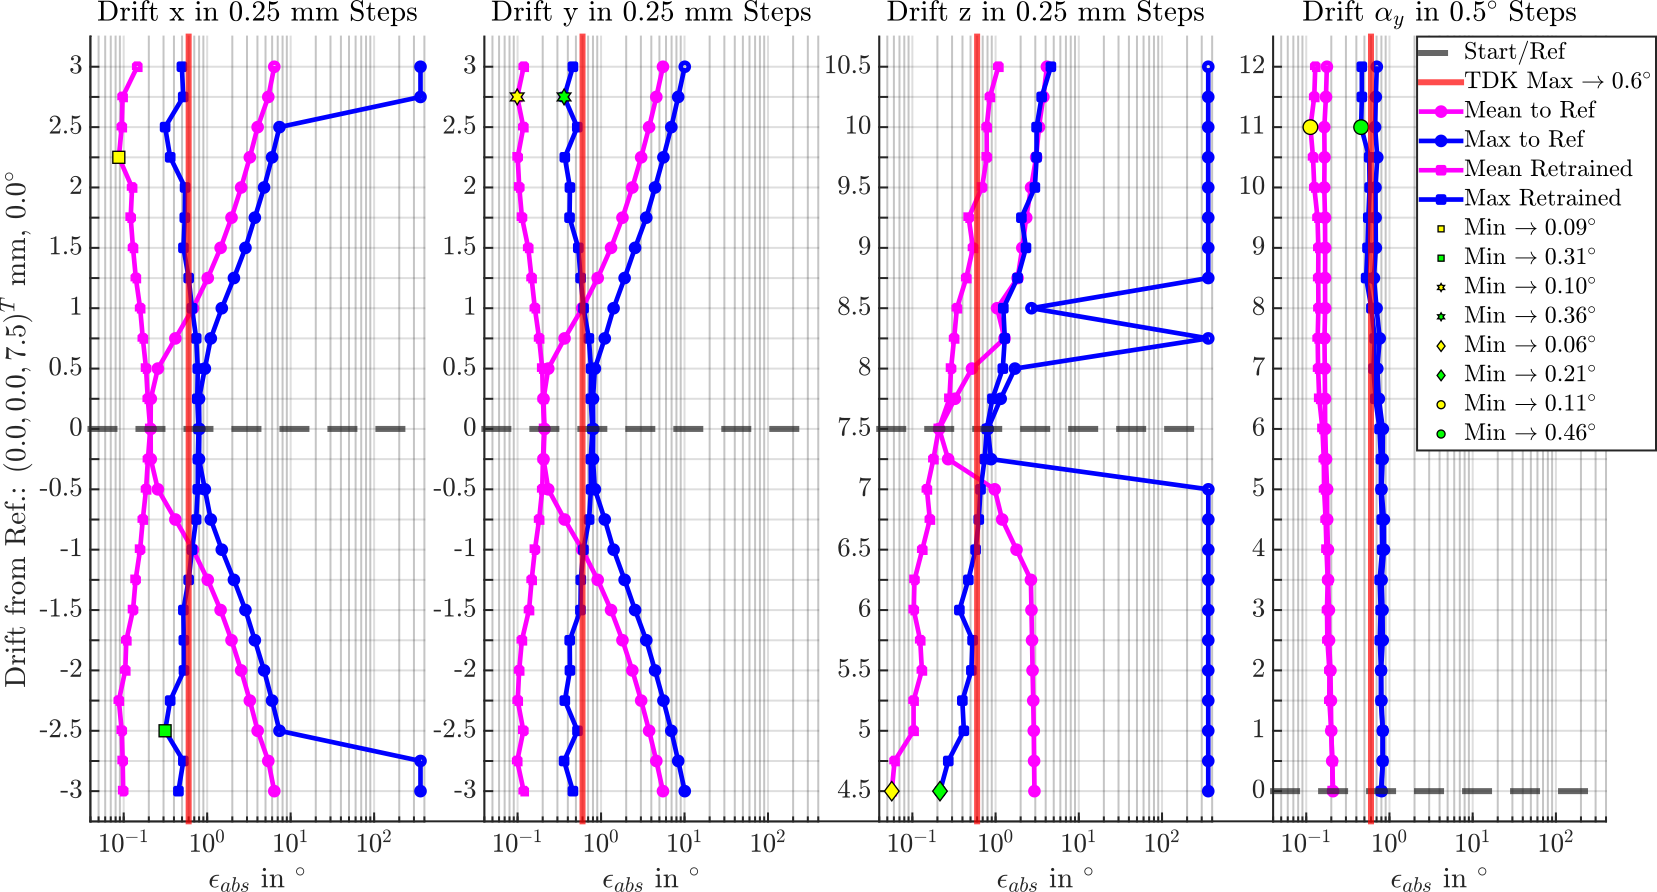
\includegraphics[width=\linewidth]{chapters/images/4-EuOExp/Drift-Model-Errors}
	\caption[Drift xyz tilt mean max errors 2 ref and retrained]{Drift xyz tilt mean max errors 2 ref and retrained}
	\label{fig:drift-model-errors}
\end{figure}
\end{landscape}


\clearpage
\begin{landscape}
\begin{figure}[tbph]
	\centering
	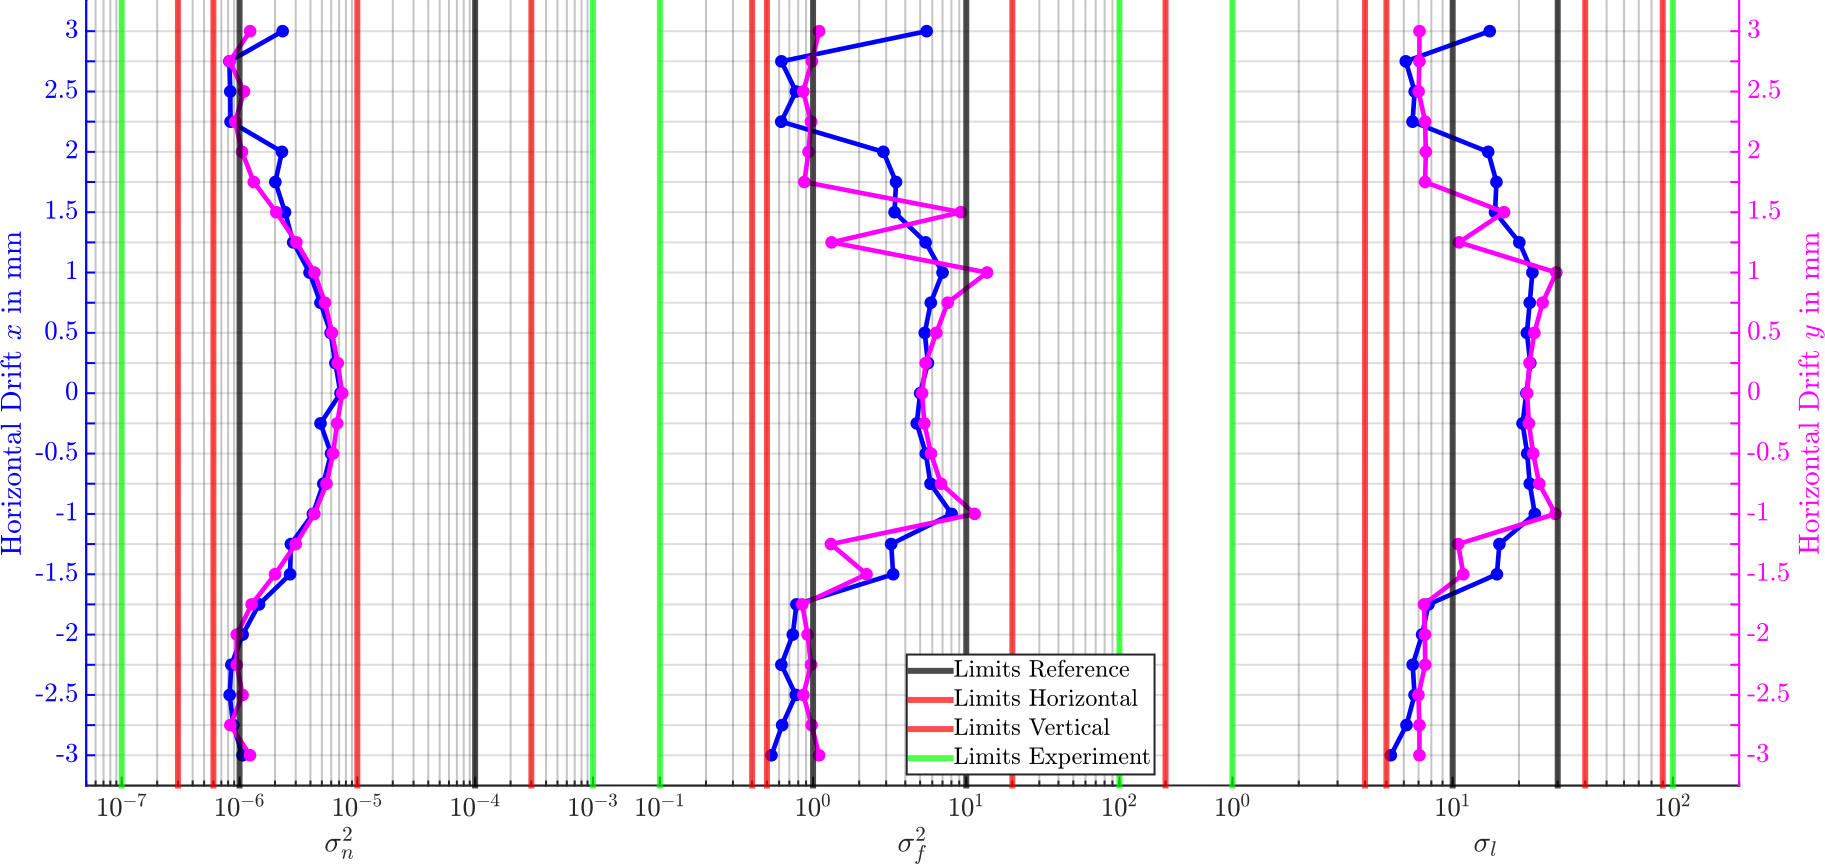
\includegraphics[width=\linewidth]{chapters/images/4-EuOExp/Drift-Horizontal-Model-Parms}
	\caption[Drift xyz tilt retrained model params tracking]{Drift xy retrained model params tracking, limits from exp and ref and new suggestion}
	\label{fig:drift-horizontal-model-parms}
\end{figure}
\end{landscape}

\clearpage
\begin{landscape}
	\begin{figure}[tbph]
		\centering
		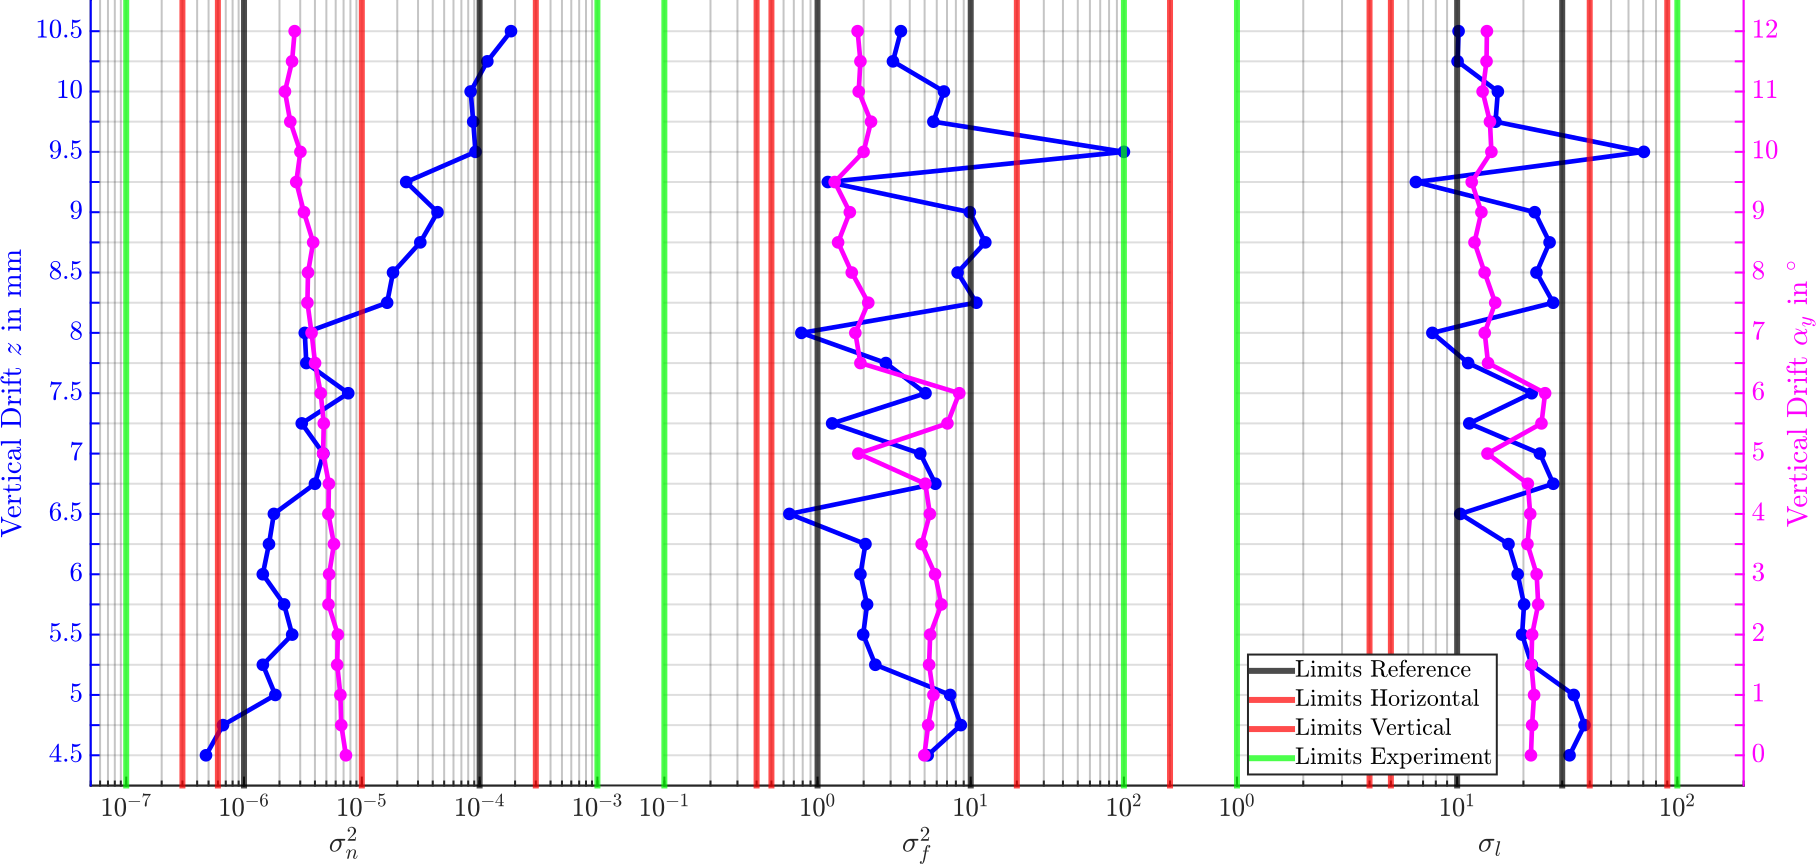
\includegraphics[width=\linewidth]{chapters/images/4-EuOExp/Drift-Vertical-Model-Parms}
		\caption[Drift xyz tilt retrained model params tracking]{Drift z tilt retrained model params tracking, limits from exp and ref and new suggestion}
		\label{fig:drift-vertical-model-parms}
	\end{figure}
\end{landscape}

\clearpage
\begin{figure}[tbph]
	\centering
	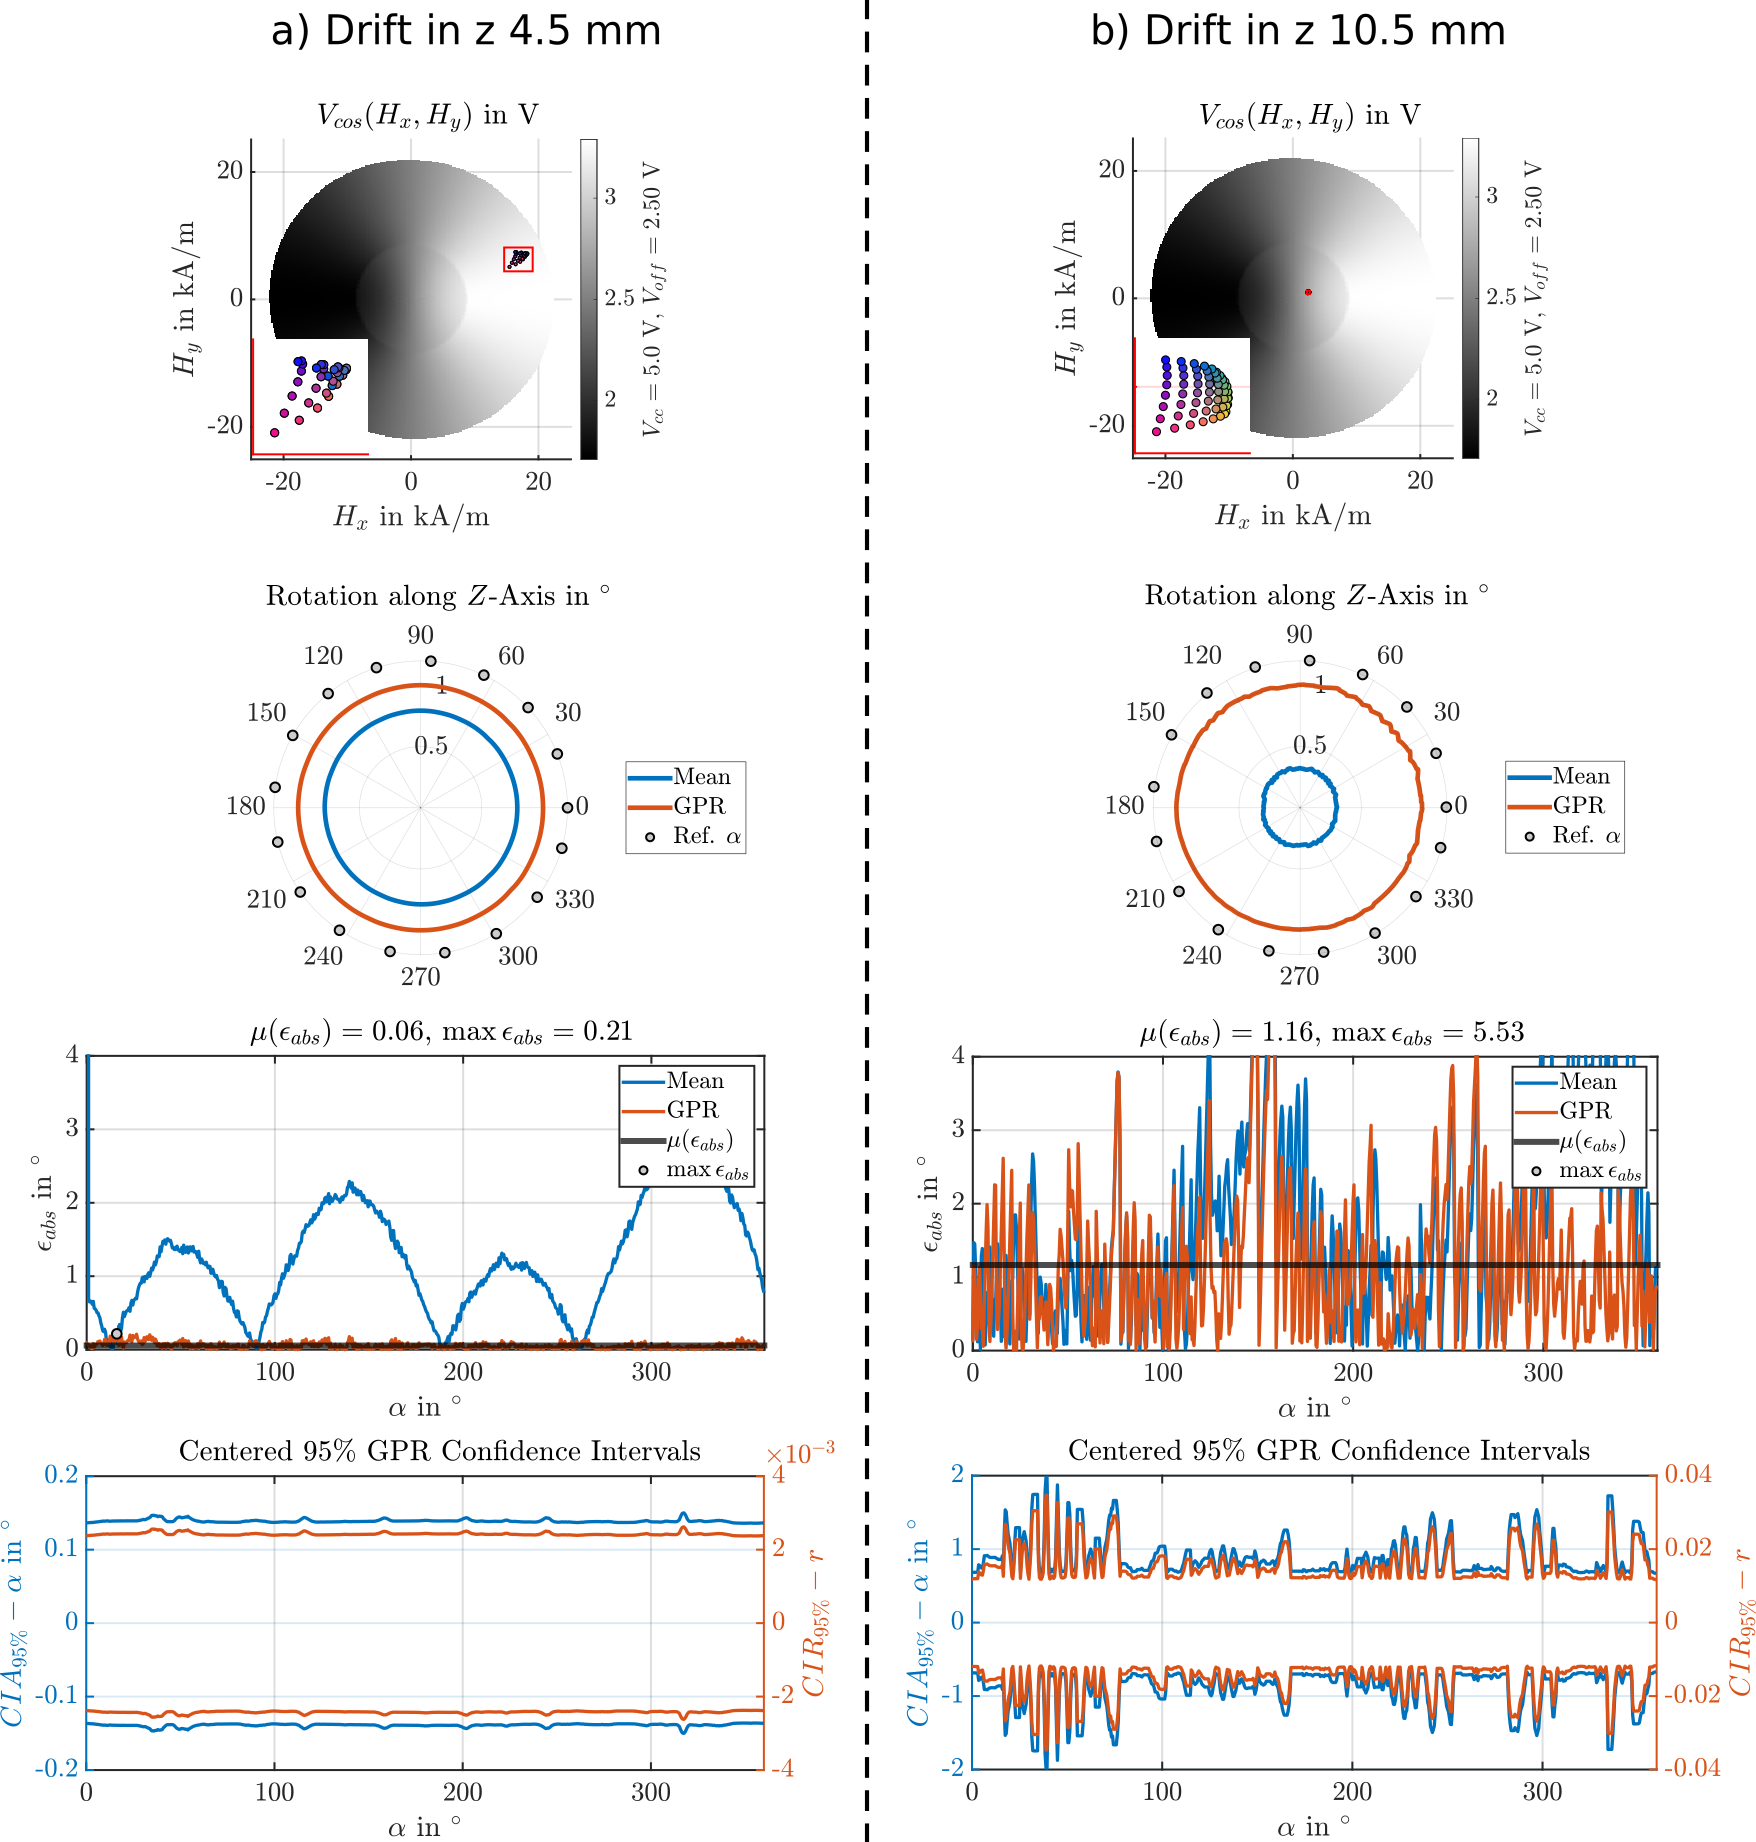
\includegraphics[width=\linewidth]{chapters/images/4-EuOExp/Z-Pos-Comp-45-105-Rotation}
	\caption[Zpos 45 105 comp rotation]{Zpos a) 45 b) 105 comp rotation $\SI{21,5}{\degree}$ comp char spredding}
	\label{fig:z-pos-comp-45-105-rotation}
\end{figure}


\clearpage


% !TEX root = ../thesis.tex
% testing and optimization experiments
% @author Tobias Wulf
%

\section{Verhalten bei kombinierten Fehllagen}\label{sec:exp6}

\textbf{Zweck:}

\textbf{Durchführung:}

\textbf{Erzeugte Datensätze:}

\textbf{Matlab-Skript:}

\textbf{Abweichende Parameter von \autoref{tab:sim-params-exp}:}

Abweichende Parameter:

Referenzposition (0,0,4.5) , 11deg 

\begin{itemize}
	\item TrainingsOptions: nAngles: 17
	\item TrainingsOptions/ TestOptions: xPos/ yPos: $(0;0)/(0,5;1)/(2,5;2)$
	\item TrainingsOptions/ TestOptions: zPos: $4,5$
	\item TrainingsOptions/ TestOptions: tilt: $11$
	\item GRPOptions: kernel : 'QFCAPX'
	\item $\sigma_f^2$-Bounds: $(0.4,20)$
	\item $\sigma_l$-Bounds: $(4,50)$
	\item $\sigma_n^2$-Bounds: $(3\cdot10^{-7},10^{-5})$
	\item GPROptions: mean: 'zero'
	\item OptimRuns 10
\end{itemize}

\textbf{Ergebnisse:}

\textbf{Beobachtungen:}


\clearpage
\begin{figure}[tbph]
	\centering
	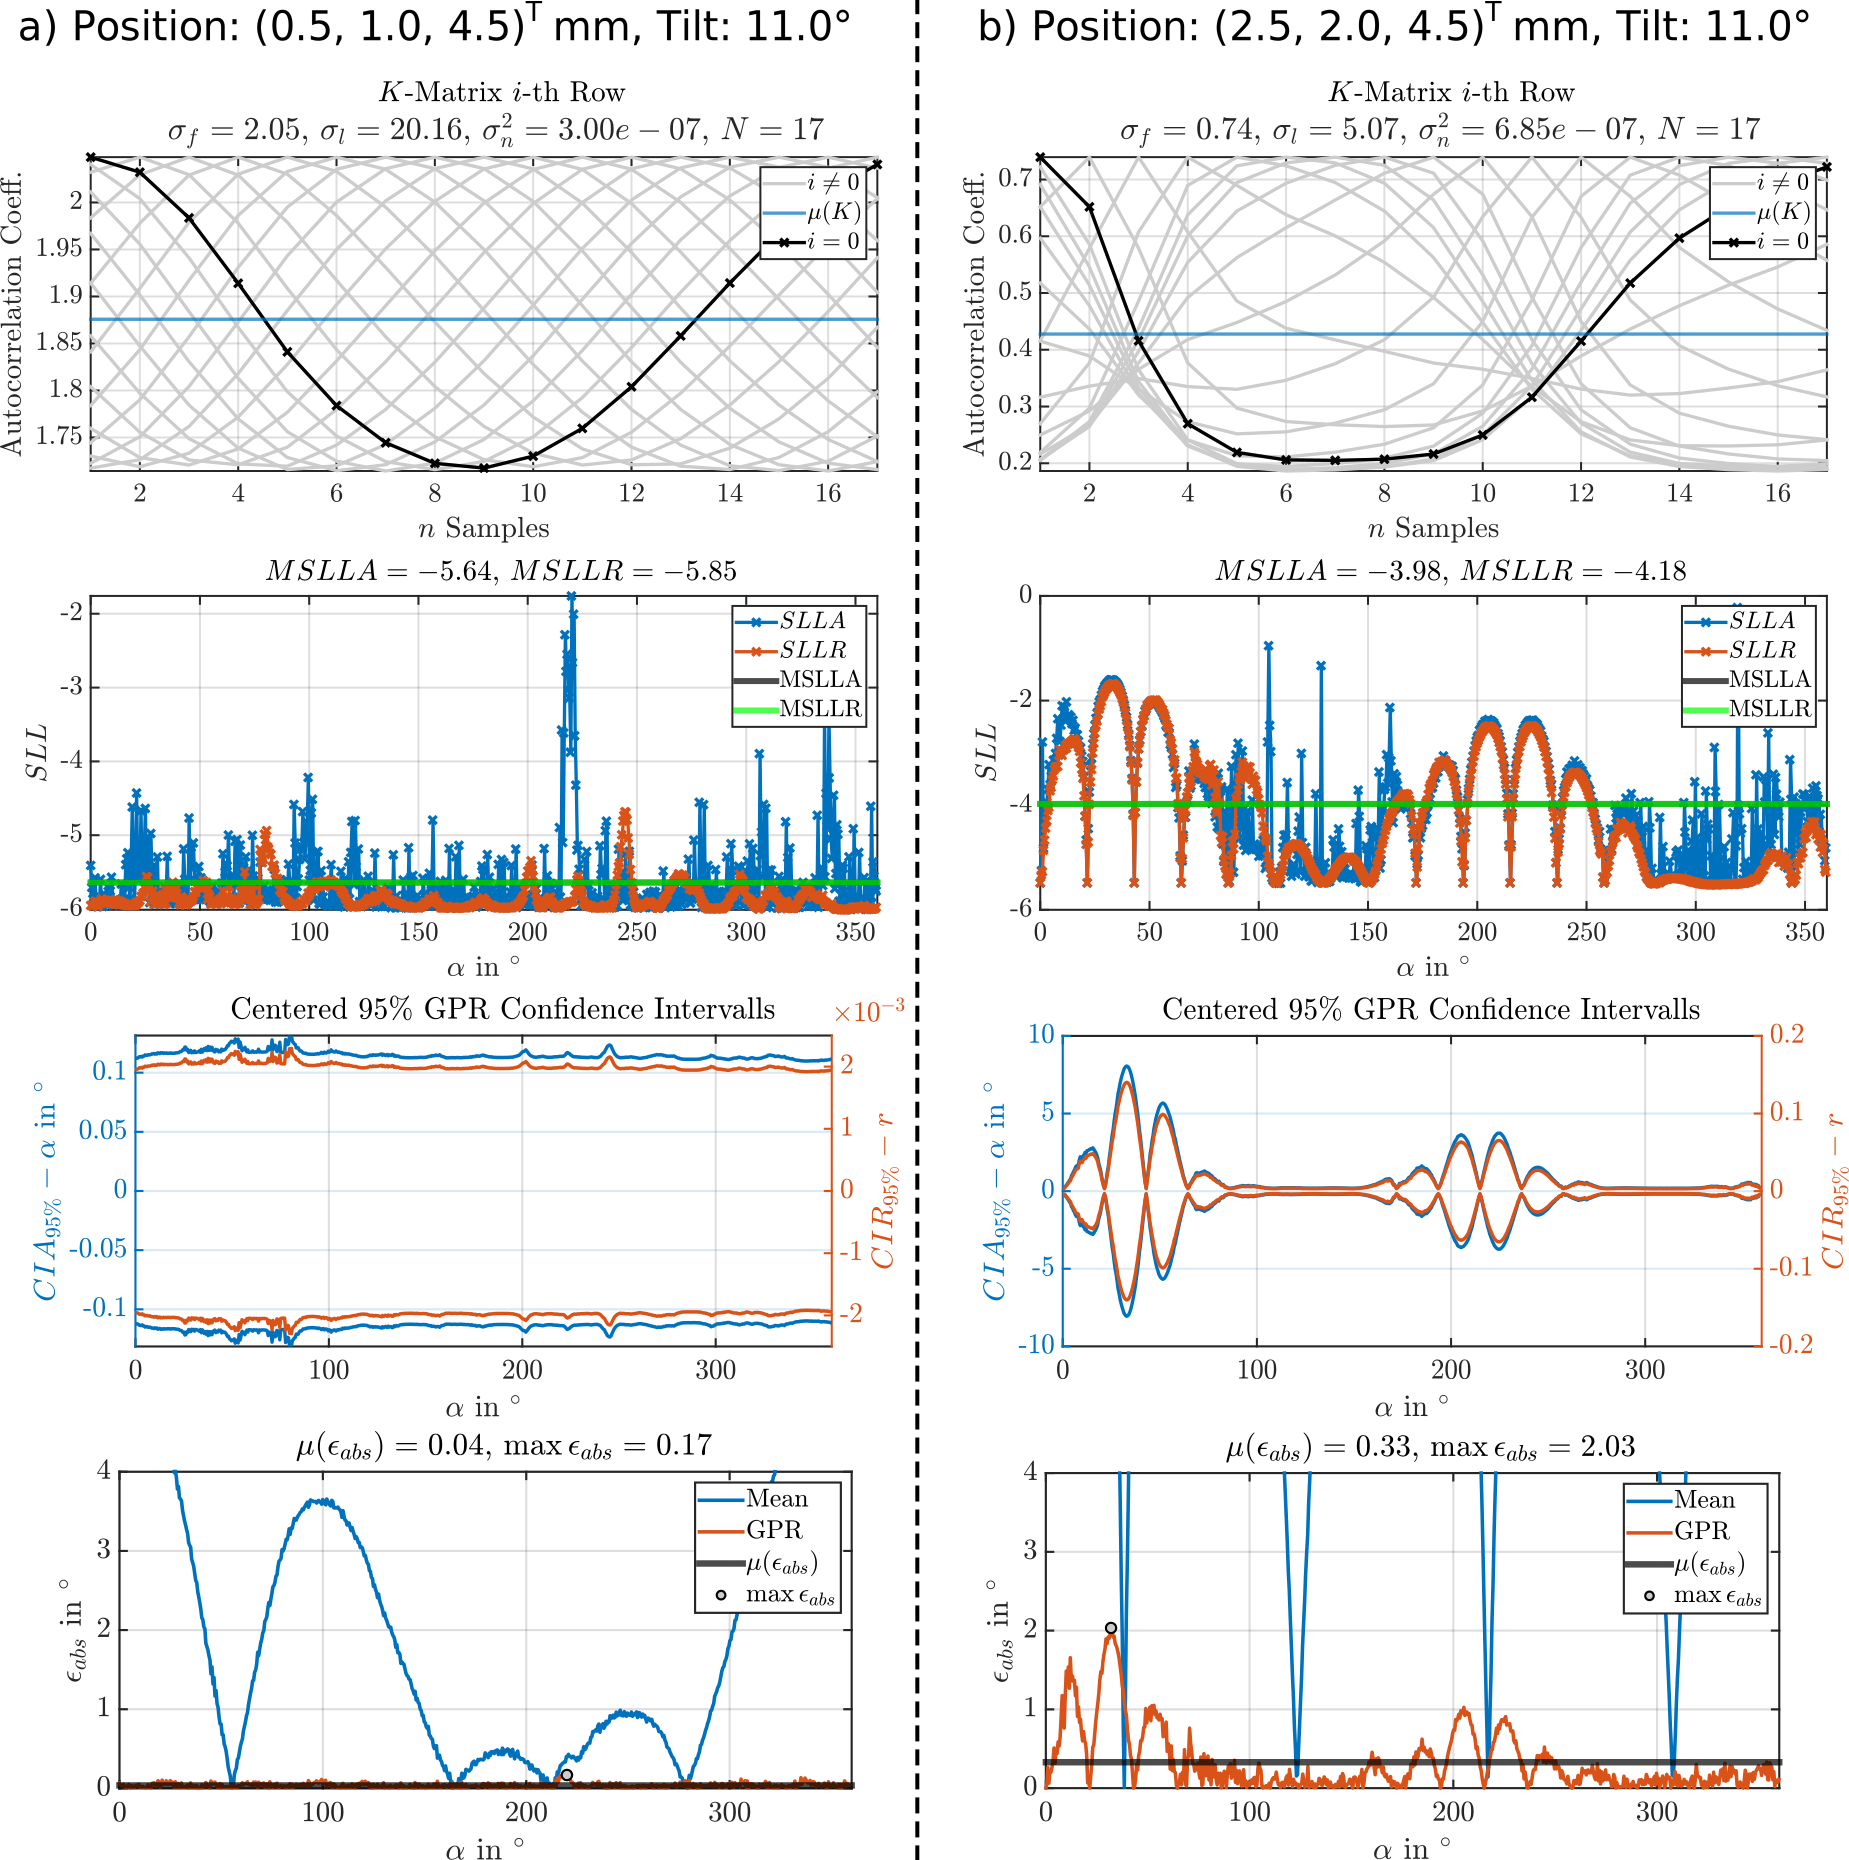
\includegraphics[width=\linewidth]{chapters/images/4-EuOExp/Kombinierte-Fehllagen-GPR}
	\caption[Kombinierte Fehllagen Modell]{Kombinierte Fehllagen Modell}
	\label{fig:kombinierte-fehllagen-gpr}
\end{figure}


\clearpage
\begin{landscape}
\begin{figure}[tbph]
	\centering
	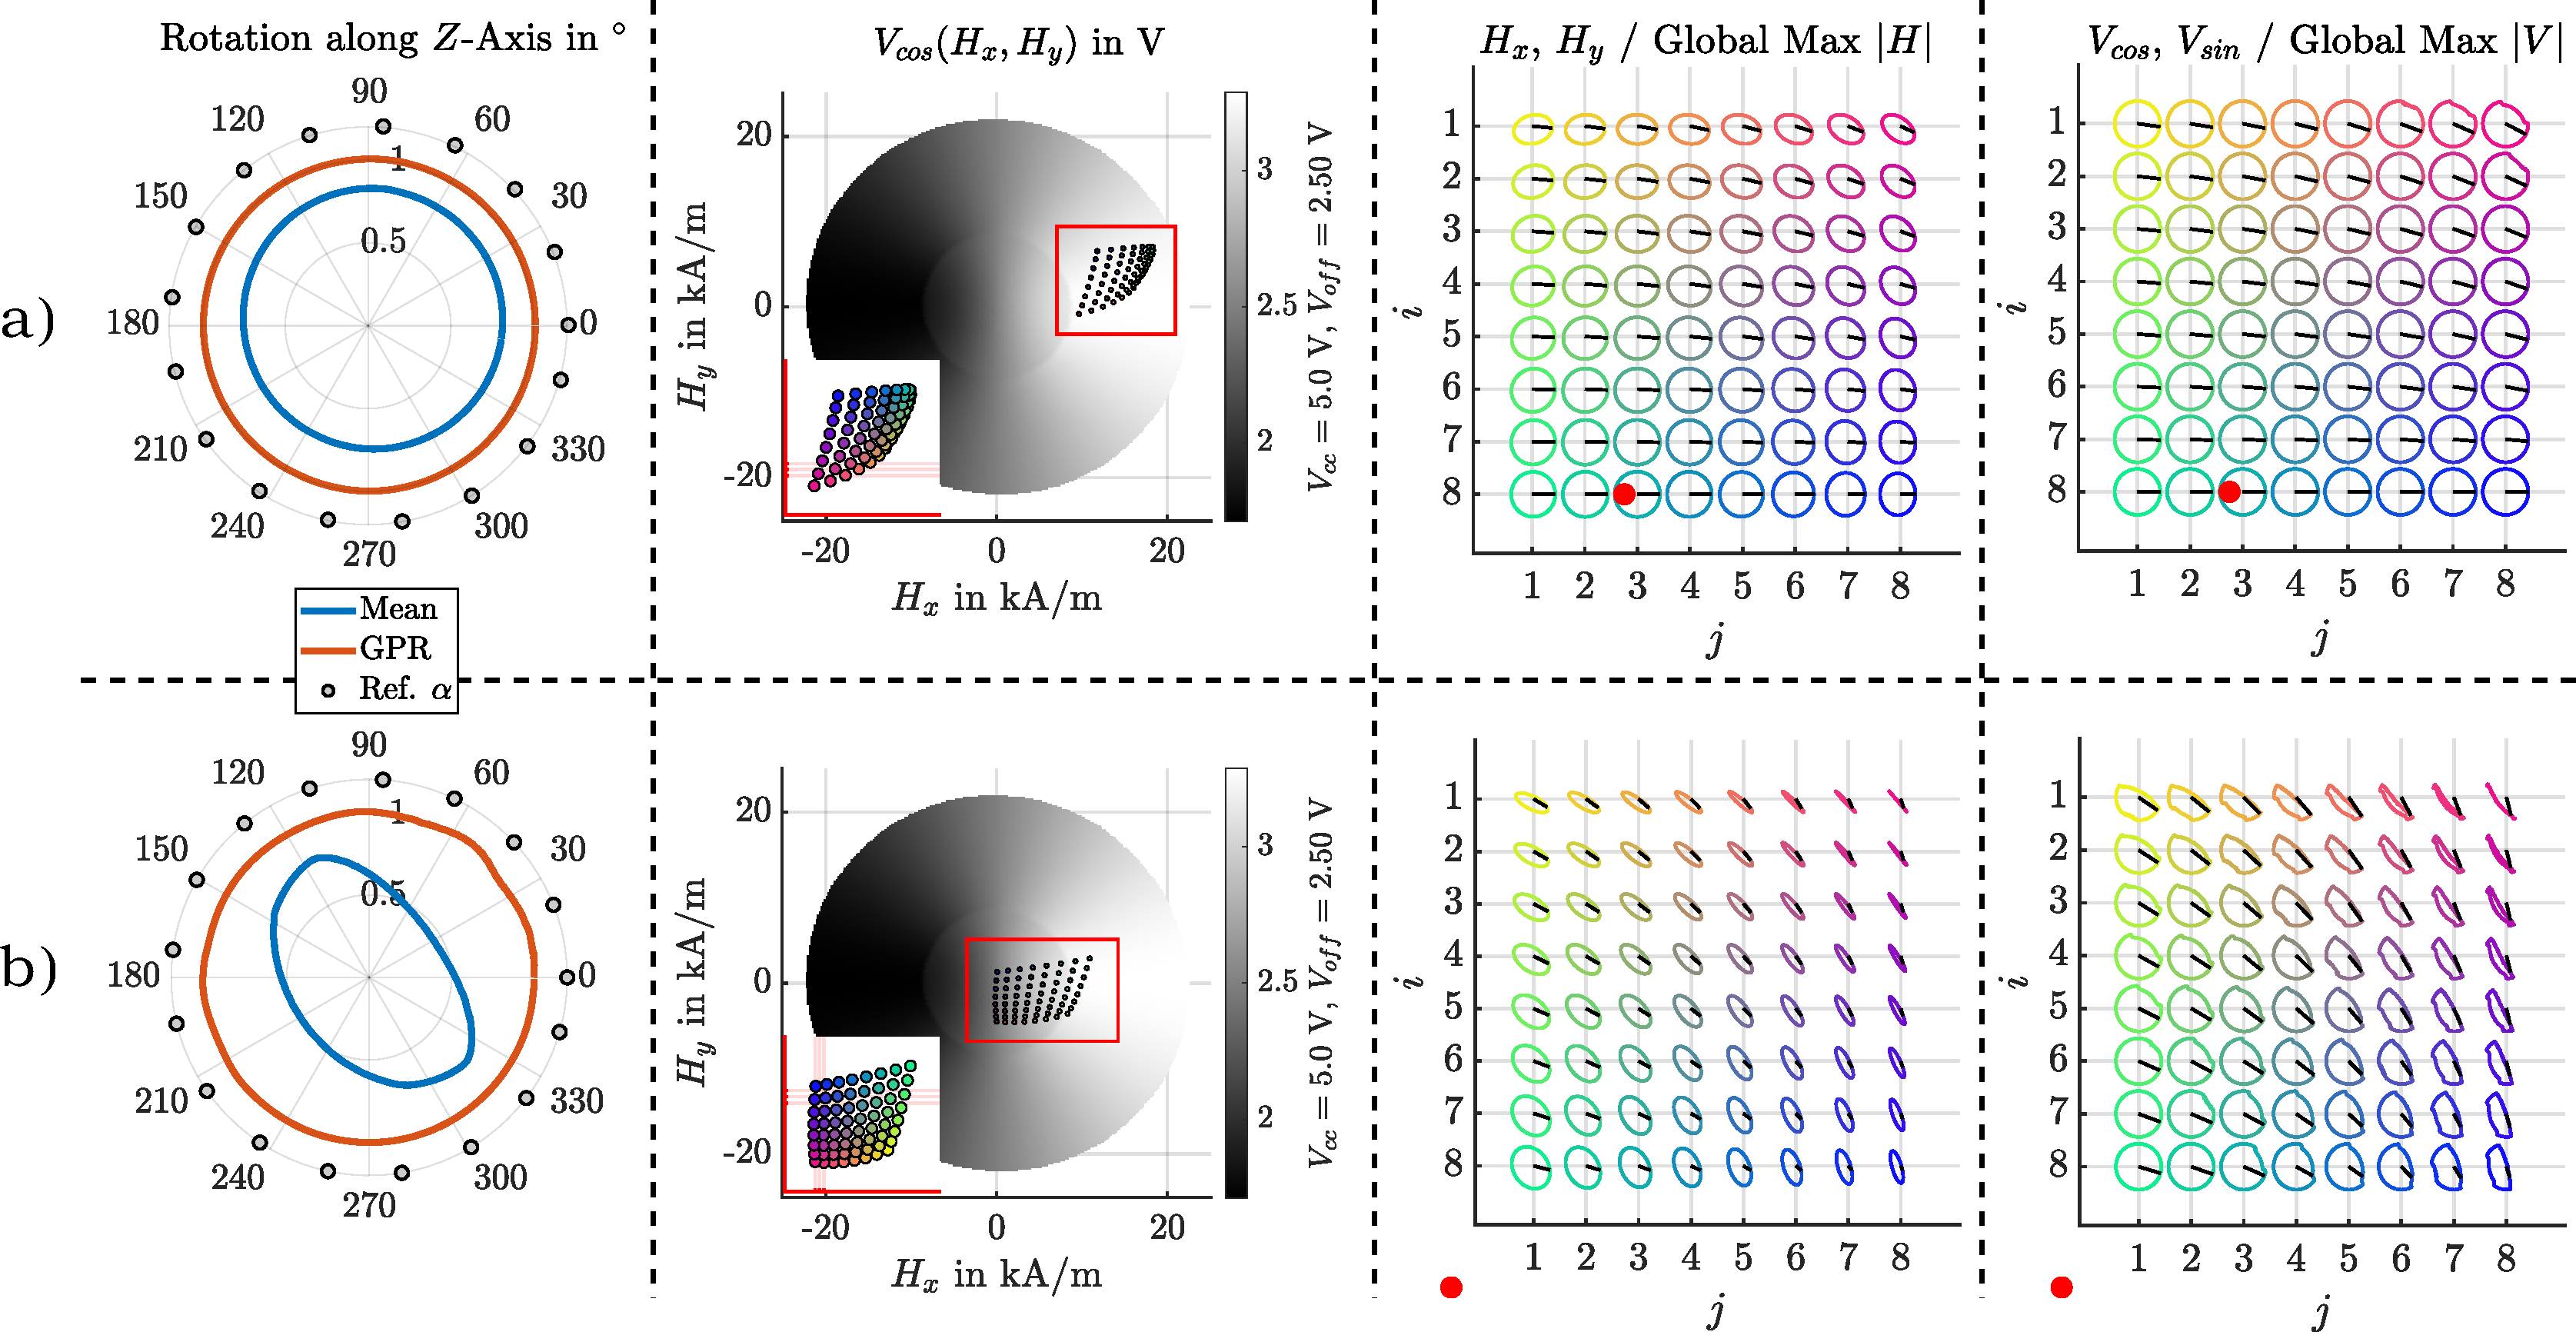
\includegraphics[width=\linewidth]{chapters/images/4-EuOExp/Kombinierte-Fehllagen-Sensor}
	\caption[Kombinierte Fehlagen Sensor]{Kombinierte Fehlagen Sensor beide 11 tilt a) (0,0,4.5) b) (2.5,2,4.5) Verzerrung}
	\label{fig:kombinierte-fehllagen-sensor}
\end{figure}	
\end{landscape}


\clearpage



